\chapter{Implementación}

\section{Elección de herramientas} \label{sec:tools}
Una vez realizada la elección de modelos en el apartado anterior \ref{ch:design}, la
elección de las herramientas es un proceso mucho más sencillo, ya que hemos establecido
los criterios que nos ayudarán a escoger aquella que se adapte mejor a las necesidades
de nuestro proyecto (en este caso de la aplicación web).

\subsection{Framework para desarrollo web}

    \subsubsection{Ruby on Rails}
    \textbf{Ruby on Rails} (también conocido como Rails) \cite{ruby-on-rails} es un framework
    para la creación de aplicaciones web escrito en Ruby. Sigue una arquitectura
    (Model-View-Controller) y diseño RESTfull\footnote{Un servicio es RESTfull cuando cumple
    con la \textbf{arquitectura REST}, es decir, facilita el acceso a recursos remotos y
    además define las operaciones típicas por medio de URIs (listar, crear, leer, actualizar
    y borrar).}. Está diseñado para facilitar la programación web al hacer una estimación
    de los componentes principales que se necesitan para comenzar.\\

    Este software asume que hay una mejor forma de hacer las cosas y está diseñado para
    ello, por lo que es un código muy optimizado y hecho para aumentar la productividad
    si se hace el desarrollo de la forma "The Rails Way".

    \subsubsection{Django}
    \textbf{Django} \cite{django} es el framework para Python más usado, está enfocado a sitios
    basados en bases de datos. Permite un desarrollo software muy rápido y limpio. Tiene una
    arquitectura MTV (Model-Template-View), donde el View sería el equivalente a Controller
    en MVC. El esquema básico de este patrón es el siguiente:

        \begin{figure}[H]
            \centering
            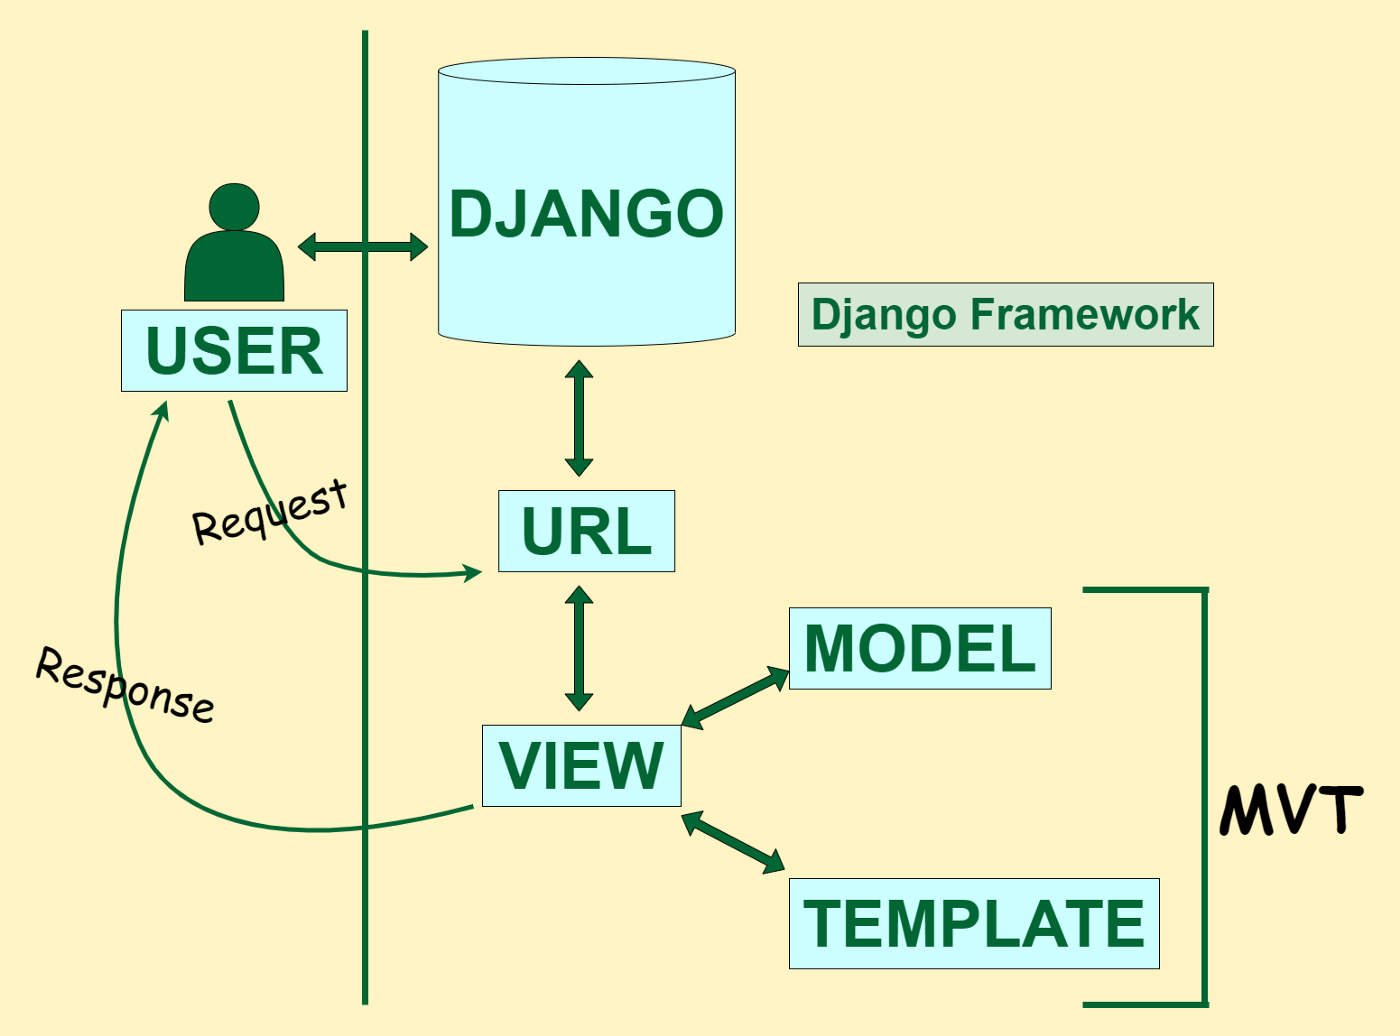
\includegraphics[scale=0.22]{imagenes/mvt.png}
            \caption[Patrón Modelo-Plantilla-Vista]{Patrón Modelo-Plantilla-Vista. Fuente \cite{mvt}}
            \label{fig:mvt}
        \end{figure}

    Como vemos, el flujo de comunicación entre estos tres bloques sería el siguiente:
        
       \begin{enumerate}
           \item El usuario interacciona con la interfaz, solicitando una url.
           \item El framework de Django, a través de su archivo urls.py, se encarga de
           decidir que \textbf{vista} se debe mostrar.
           \item Si dicha vista obtiene datos de la base de datos, ésta se comunica con el 
           \textbf{modelo}.
           \item Finalmente, se devuelve la \textbf{plantilla} con los datos de la base de datos si
           fuera necesario.
       \end{enumerate}

    Al igual que el anterior framework mencionado, Django ha sido diseñado por programadores
    experimentados, y se encarga de las partes más complejas del desarrollo web, permitiendo
    que el programador se centre en escribir la aplicación sin necesidad de preocuparse
    por otras cuestiones.

    \subsubsection{Laravel}
    \textbf{Laravel} \cite{laravel} es el mejor framework de PHP para desarrollar aplicaciones
    y servicios web con PHP5, PHP7 y PHP8. Al igual que Ruby on Rails, sigue una arquitectura 
    MVC, por lo que es sencillo relacionar las distintas componentes de la aplicación.\\

    Es un framework moderno que ofrece muchas utilidades a los desarrolladores y permiten un
    desarrollo ágil de las aplicaciones web. Además, pone mucho interés en la calidad del
    código, el mantenimiento y la escalabilidad.

    \subsubsection{Angular}
    \textbf{Angular} \cite{angular} es un framework desarrollado en TypeScript para el
    desarrollo de aplicaciones web. Está mantenido por Google, utilizado para crear y mantener
    aplicaciones SPA (Single Page Application), es decir páginas web que interaccionan con el
    usuario dinámicamente sobreescribiendo la página con información nueva.\\

    Al contrario que los frameworks anteriormente mencionados, Angular no usa un modelo MVC
    o MVT, sino que permite el desarrollo del front-end y el back-end de forma totalmente
    independiente.

\subsection{Framework CSS}

    \subsubsection{Tailwind CSS}
    \textbf{Tailwind CSS} \cite{tailwind-css} es un framework CSS que funciona escaneando los
    archivos HTML, componentes Javascript y otros templates generando los correspondientes
    estilos y escribiéndolos en un archivo CSS estático. No tiene muchos componentes, sino
    clases de utilidad que pueden aplicarse directamente sobre el código HTML del proyecto.
    Además de esto, permite una gran optimización del peso del código CSS mediante unos flujos
    de desarrollo.
        
    \subsubsection{Bootstrap}
    \textbf{Bootstrap} \cite{bootstrap} es uno de los frameworks más populares y usados para
    el desarrollo de páginas web. Fue desarrollado por Twitter en 2010 para uso de la compañía
    pero más tarde pasó a ser código abierto. Este framework combina CSS y Javascript. Entre
    sus características fundamentales podemos encontrar:
    
    % \begin{list}{\textbullet}{ 
        %     \addtolength{\labelsep}{1mm}    % Distancia hasta la etiqueta
        %     \addtolength{\itemsep}{-2mm}    % Separación entre items
        %     \setlength{\itemindent}{5mm}}   % Identación de los items
        % \end{list}
        
        \begin{itemize}
            \item \textbf{Responsive design (diseño adaptativo)}: adaptación automática a
            distintos dispositivos como móviles y tablets.
            \item \textbf{Grid System (sistema de rejilla)}: posicionamiento de elementos en
            la página.
            \item \textbf{Interface UI (interfaz de usuario)}: incluye formularios, botones,
            menús, etc.
        \end{itemize}
        
        \subsubsection{Foundation}
        \textbf{Foundation} \cite{foundation} es el principal competidor de Bootstrap, es
        un framework orientado al desarrollo de sitios web totalmente adaptativos bajo el
        enfoque \textit{mobile first}, que es una metodología de desarrollo donde se tiene
        en cuenta en primer lugar los dispositivos móviles. Esta metodología es totalmente
        contraria a la que usa Bootstrap ya que en él se usa \textit{Responsive Web Design}
        y en éste \textit{Mobile First Web Design}.\\
        
        Además de su metodología de desarrollo, posee ciertas características muy interesantes:
        
        \begin{itemize}
            \item \textbf{Fastclick}: eliminación del retraso al pulsar en dispositivos
            móviles.
            \item \textbf{Semántico}: todo es semántico, permitiendo tener un lenguaje de
            marcado limpio sin sacrificar su funcionalidad y velocidad.
            \item \textbf{Off Canvas}: creación de menús dinámicos
            \item \textbf{Customizable}: permite hacer diseño completamente personalizables,
            pudiendo eliminar elementos, definir el tamaño de las columnas, colores,
            fondos, etc
        \end{itemize}

    \subsubsection{Materialize CSS}
    \textbf{Materialize CSS} \cite{materialize-css} sigue el principio \textit{Material Design},
    es decir, ofrece componentes ya listos para ser utilizados, por supuesto adaptativo.
    Además, integra comportamientos dinámicos mediante JavaScript y no necesita de Jquery para
    funcionar.\\

    Entre sus principales características se encuentran:
        
        \begin{itemize}
            \item Al igual que otros frameworks mencionados, permite un diseño adaptativo.
            \item Permite crear menús laterales desplegables o abiertos según la resolución
            del dispositivo.
            \item Diseños utilizando la filosofía Material Design (colecciones, tarjetas,
            barras de navegación, modales, toast, etc).
            \item Añade utilidades como \textbf{Parallax} (técnica de diseño web en la que se crea
            un efecto de profundidad al hacer scroll)
        \end{itemize}

\subsection{Base de Datos}
Los distintos SGBD (Sistemas Gestores de Bases de Datos) datos que podemos encontrar son los
siguientes:

    \subsubsection{MySQL}
    \textbf{MySQL} \cite{mysql} es un sistema de gestión de bases de datos relacionales de
    código abierto (también conocido como RDBMS, Relational Database Management System). Es
    una de las bases de datos más populares en la actualidad y usa un modelo
    cliente-servidor.
    

    \subsubsection{SQLite}
    \textbf{SQLite} \cite{sqlite} es un RDBMS de tamaño reducido (aproximadamente 275 kiB)
    que a diferencia de otros RDBMS como mySQL, no usa un proceso cliente y un proceso
    servidor(modelo cliente-servidor). En este caso, funciona como un servidor
    propio independiente, haciendo uso de llamadas a subrutinas y funciones integradas en el
    propio código fuente que eliminan la necesidad de hacer consultas entre procesos
    separados.

    \subsubsection{PostgreSQL}
    \textbf{PostgreSQL} \cite{postgresql} es un sistema de gestión de base de datos relacional
    que está orientado a objetos, de código abierto y además gratuito. Este RDBMS posee tipos
    de datos avanzados y permite optimizar de forma considerable el rendimiento, este tipo de
    características por lo general solo se ofrecen en sistemas de bases de datos privativas.
    Además de las características anteriormente mencionadas, permite un control de grandes
    volúmenes de datos y tiene soporte completo para \textbf{ACID} (\textit{Atomicity,
    Consistency, Isolation, Durability}).

\subsection{Soluciones propuestas}
Como se ha mencionado anteriormente, en cualquier elección de herramientas se debe señalar
claramente las características que debe cumplir para así poder descartar con facilidad
entre las disintas alternativas.

    \subsubsection{Elección del Framework de Desarrollo Web}
    El framework de Desarrollo Web debe cumplir con una serie de \textbf{requisitos} para
    su aceptación:

        \begin{enumerate}
            \item Que siga un patrón Modelo-Vista-Controlador \ref{sec:mvc}.
            \item Que haga una deducción de los elementos principales de la aplicación,
            permitiendo centrarnos exclusivamente en el desarrollo de la misma.
            \item Que pueda permitir la configuración del mismo con distintas bases de
            datos.
            \item Que posea un sistema de gestión de usuarios (\textbf{autenticación}).
            \item Que el manejo de los modelos de la base de datos pueda abstraerse
            independientemente de la base de datos elegida mediante un \textbf{Object
            Relational Mapping} (ORM).
            \item Que incluya una fácil creación de la API para la posible comunicación
            con la App android.
        \end{enumerate}

    Tras tantear los distintos frameworks para el desarrollo de aplicaciones web disponibles
    se ha decidido utilizar Django, ya que está hecho en un lenguaje familiar para mí y
    además cumple todos los requisitos anteriormente mencionados.\\

    Dicho framework permite hacer lo siguiente:
        
        \begin{itemize}
            \item Crear la aplicación sin tener que preocuparnos de elementos para que
            ésta funcione.
            \item Configuración con distintas bases de datos, SQLite es la base de datos
            por defecto, pero además permite configurarlo para trabajar con mySQL y
            postgreSQL.
            \item Sistema de autenticación de usuarios, por lo que podremos gestionar el
            registro e inicio de sesión de los mismos.
            \item Contiene un ORM que permite el manejo de modelos de la base de datos
            abstrayendo la base de datos utilizada.
            \item A pesar de no venir incluido como tal, instalando la aplicación Django
            REST framework, es posible realizar la configuración de la API de una forma
            relativamente sencilla.
            \item Tiene una documentación realmente buena, clara y sencilla.
        \end{itemize}
    
    Éstas son las razones por las que se ha decidido elegir Django para el desarrollo de
    nuestra aplicación web.

    \subsubsection{Elección del Framework CSS}
    Entre los requisitos que el framework CSS debe cumplir están los siguientes:

        \begin{enumerate}
            \item Que permita un diseño adaptativo de la página web.
            \item Que siga la metodología Responsive Web Design.
            \item Que sea fácil de usar.
            \item Que esté actualmente mantenido por la comunidad.
            \item Que posea una documentación simple y fácil de entender. 
        \end{enumerate}

    Siguiendo los requisitos de arriba, Foundation puede ser descartado ya que no cumple el
    segundo requisito, ya que nuestra aplicación web principalmente va a estar diseñada para
    utilizarse en un ordenador (también podrá usarse en un smartphone, pero no es la
    finalidad).\\

    Entre los tres frameworks restantes, podría utilizarse cualquiera de ellos ya que
    cumplen con los requisitos, pero finalmente se ha decidido utilizar Bootstrap ya que
    es probablemente el framework más popular y sencillo de usar que hay, además de seguir
    siendo muy usado por la comunidad. 
    

    \subsubsection{Elección de la Base de Datos}
    Para la elección de la Base de Datos que utilizará el servidor web para almacenar toda
    la información de las excavaciones se tienen que cumplir los siguientes requisitos:

        \begin{enumerate}
            \item Que sea una base de datos relacional.
            \item Que sea open-source y gratuita.
            \item Que tenga soporte para la realización de transacciones seguras.
            \item Que haga un uso eficiente de los datos.
        \end{enumerate}

    Por cuestiones de escalabilidad, utilizar SQLite se puede descartar ya que posee un
    reducido número de tipos de datos y más bien está pensada para utilizarse en dispositivos
    con poca capacidad de almacenamiento.\\

    Ahora nos tocaría pensar en, ¿mySQL o postgreSQL? Realmente podría utilizarse cualquiera
    de las dos, pero postgreSQL ofrece algunas ventajas respecto a mySQL que merece la pena
    mencionar: 
    
        \begin{itemize}
            \item MySQL es propiedad de Oracle y podría pasar a ser un producto comercial
            (de pago), sin embargo, postgreSQL es \textbf{open source 100\%}.
            \item PostgreSQL ofrece una mayor \textbf{integridad y fiabilidad} de los datos
            (principio ACID).
            \item Gracias a funciones que lectura y escritura en paralelo, postgreSQL ofrece
            una mayor \textbf{velocidad} frente a mySQL.
        \end{itemize}
    
    Por estas razones, finalmente se ha decidido usar postgreSQL como base de datos para
    nuestro servidor web.

\section{Desarrollo basado en sprints} \label{sec:sprints}
Como mencionamos en el sub-apartado \ref{subsubsec:scrum}, se va a trabajar mediante
\textbf{sprints}, concepto del marco de trabajo Scrum. Es por ello que el desarrollo del
software se ha dividido en una serie de \textbf{hitos} (que en este caso serían nuestros
sprints). Un hito, en el desarrollo de software, simboliza un logro, un aspecto del proyecto
que se está cumpliendo conforme se planificó al comienzo del mismo, por tanto, éstos son los
mejores indicadores del progreso del proyecto para alcanzar los objetivos finales.\\

A cada uno de estos sprints se le irán asociando \textbf{issues} (tareas) que se deben realizar
para alcanzar el objetivo del mismo. Dichas tareas pueden ser aspectos a mejorar del software,
errores que se han encontrado, tareas referentes a documentación, etc.\\

Los hitos (\textbf{milestones}) del proyecto son los siguientes:
\begin{enumerate}
    \item \textbf{\href{https://github.com/alexespana/TFG/milestone/1}{[M1]. Website
    creation (Creación del sitio web)}}: creación de la estructura principal de la
    aplicación web, con las principales páginas y funcionalidades. Esta parte será
    desarrollada en un entorno de desarrollo (servidor de desarrollo).
    \item \textbf{\href{https://github.com/alexespana/TFG/milestone/8}{[M2]. Database
    creation (Creación de la Base de Datos)}}: creación de las principales tablas para
    modelar el problema, junto con los correspondientes formularios para la recogida de
    datos en la aplicación web.
    \item \textbf{\href{https://github.com/alexespana/TFG/milestone/2}{[M3]. Authentication
    (Autenticación)}}: gestión de usuarios del sitio web, signup, signout, login, logout,
    cambiar contraseña e información de contacto para cada usuario así como third party
    (social) account authentication. 
    \item \textbf{\href{https://github.com/alexespana/TFG/milestone/3}{[M4]. Test behavior
    (Testear comportamiento)}}: realización de tests para comprobar el comportamiento
    de la aplicación.
    \item \textbf{\href{https://github.com/alexespana/TFG/milestone/4}{[M5]. Continuous
    integration (Integración Continua)}}: el software desarrollado debe integrarse con el
    posible software ya existente en el sitio web, asegurando el correcto funcionaminto
    de ambos.
    \item \textbf{\href{https://github.com/alexespana/TFG/milestone/6}{[M6]. API REST}}:
    el diseño y posterior implementación de la API REST que permita gestionar los recursos
    con los que trabaja la aplicación.
    \item \textbf{\href{https://github.com/alexespana/TFG/milestone/5}{[M7]. Log system
    (Sistema de Log)}}: los eventos más importantes que ocurren en la aplicación deben ser
    grabados a través del uso de un servicio de log. Es conveniente capturar errores en un
    nivel superior de abstracción, evitando modificar código ya hecho.
    \item \textbf{\href{https://github.com/alexespana/TFG/milestone/7}{[M8]. Deployment
    (Despliegue)}}: el despliegue de la aplicación web en la nube debe realizarse utilizando
    un dominio público y un WSGI (Web Server Gateway Interface).
\end{enumerate}

Si desea tener una vista más general de los milestones, issues, commits, branches, etc del
proyecto puede visitar los siguientes enlaces:

\begin{itemize}
    \item \textbf{\href{https://github.com/alexespana/TFG/milestones}{Milestones (Hitos)}}
    \item \textbf{\href{https://github.com/alexespana/TFG/issues}{Issues (Tareas)}}
    \item \textbf{\href{https://github.com/alexespana/TFG/branches}{Branches (Ramas)}}
    \item \textbf{\href{https://github.com/alexespana/TFG/pulls}{Pull requests (Solicitudes
    de cambio)}}
\end{itemize}


\subsection{Creación del sitio web}
Para realizar la implementación de las distintas plantillas de la aplicación, se ha hecho
uso del sistema propio de plantillas de Django, llamado \textbf{Django template language},
que es muy parecido a JinJa2 y que está completamente implementado en los backends que
incluye de serie.\\

A la hora de pensar en un diseño para la aplicación web, se ha optado por un diseño
minimalista, que permita diferenciar fácilmente las distintas partes de la aplicación
junto con sus funcionalidades.\\

Es importante mencionar que todas las plantillas del proyecto hacen uso de una plantilla
base que contiene el navegador de la página y el pie de página, por lo que dicha plantilla base
sería tal que así:\\

    \begin{figure}[H]
        \centering
        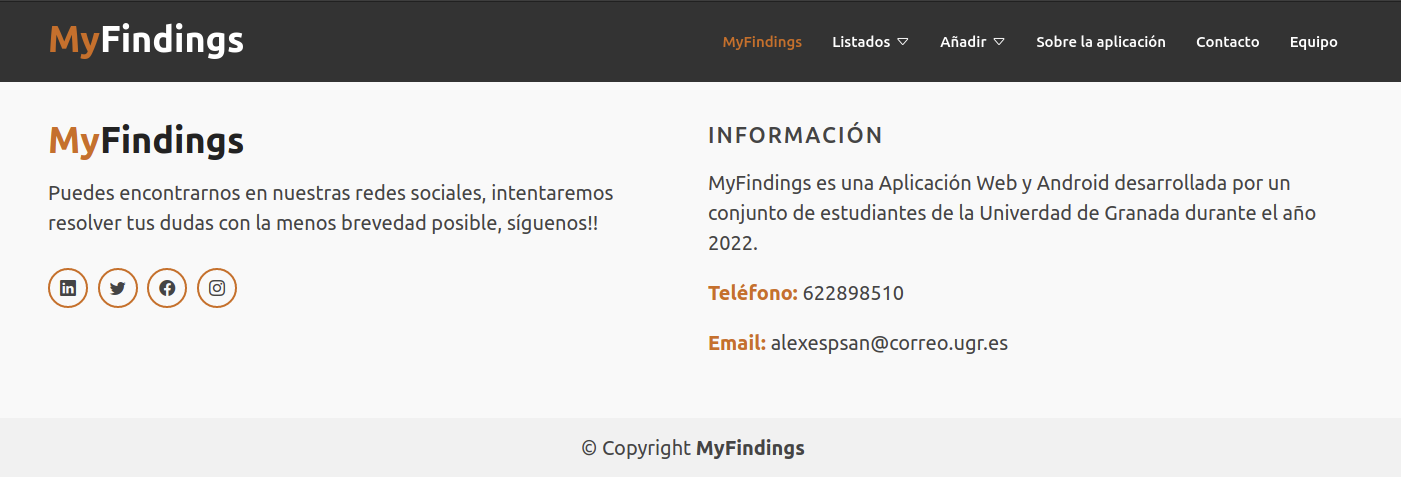
\includegraphics[scale=0.25]{imagenes/base.png}
        \caption{Plantilla base}
        \label{fig:base}
    \end{figure}

El resto de plantillas de este diseño son las que se describen en las secciones siguientes.

    \subsubsection{Home}
    Ésta es la página principal que se verá al entrar en la aplicación, prácticamente todo el
    diseño de ésta tiene relación con un componente de bootstrap llamado \textbf{Carousel}, que
    nos permite construir una especie de sliders en la vista con indicadores en la parte
    inferior. Además, cada uno de estos sliders puede tener texto asociado e imágenes de fondo,
    por lo que podemos ir cambiando el fondo completo de la página mediante el uso de javascript
    cada cierto tiempo predefinido. De esta forma, hacemos que entrar en la página sea una
    sensación agradable a primera vista. El \textbf{home} quedaría así:
    
        \begin{figure}[H]
            \centering
            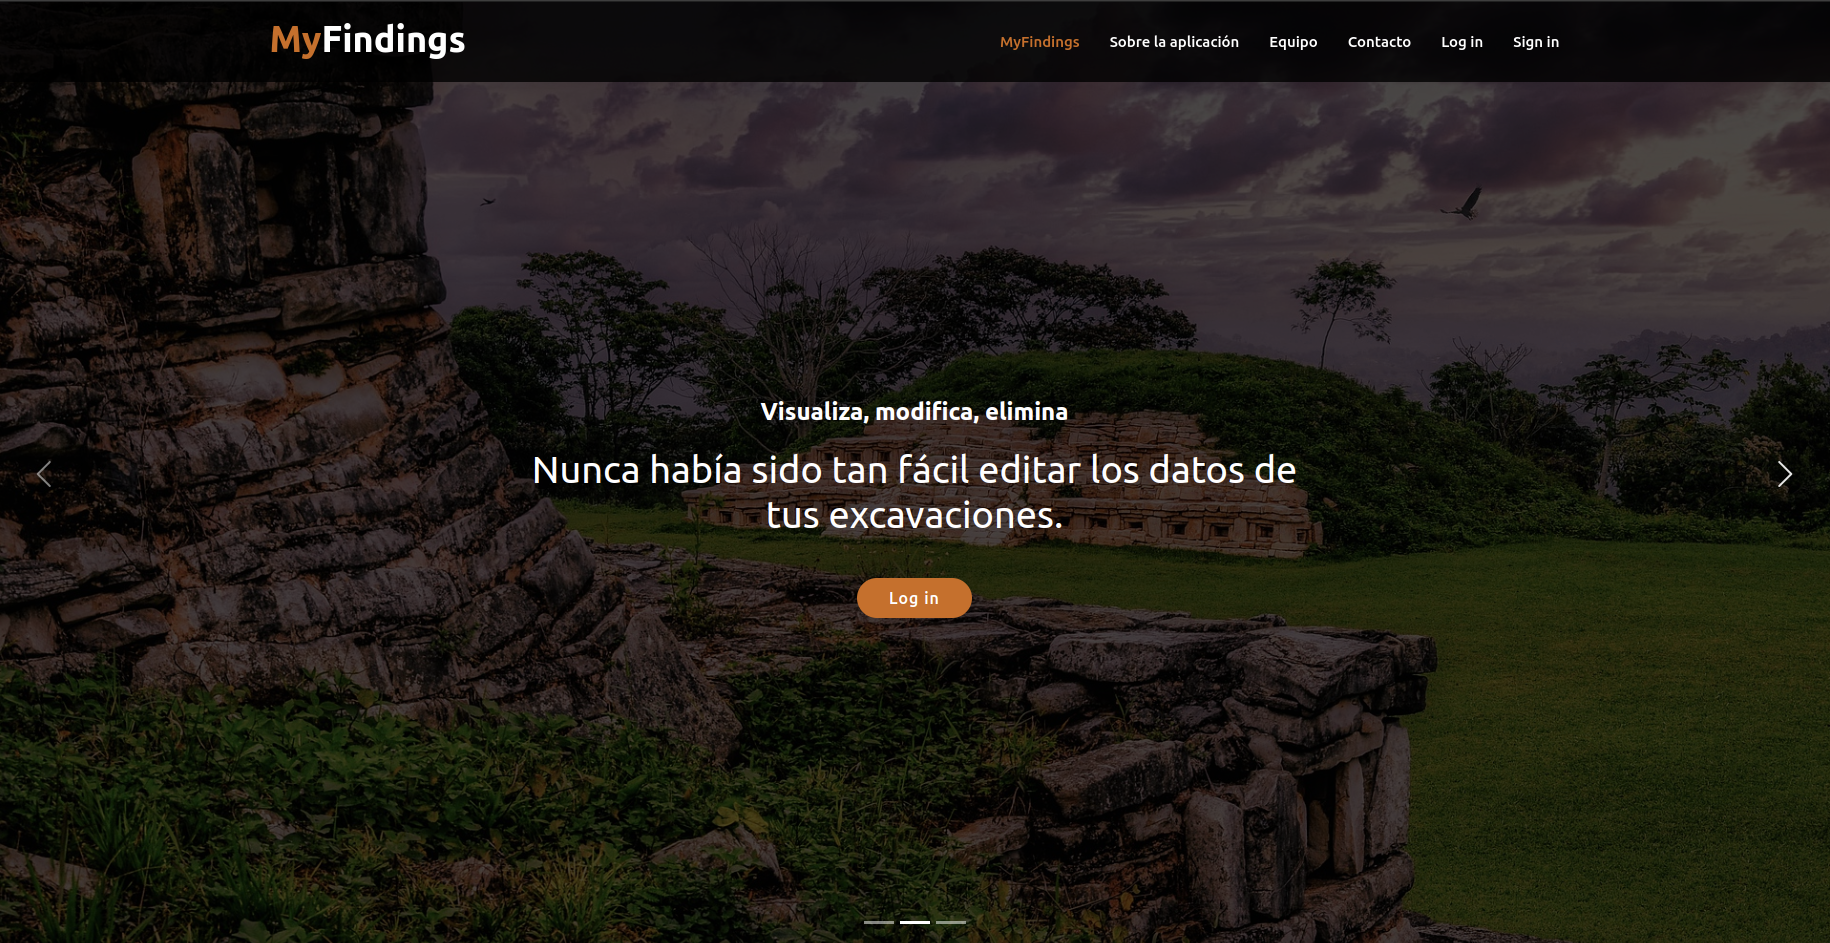
\includegraphics[scale=0.19]{imagenes/home.png}
            \caption[Home de la página]{Home de la página. Fuente \cite{maya}}
            \label{fig:home}
        \end{figure}

    \subsubsection{Listados}
    Esta parte de la vista corresponderá a distintas vistas que servirán para listar en forma
    de \textbf{tablas} las distintas excavaciones, estancias, hechos, unidades estratigráficas
    (sedimentarias y construidas), fotografías, materiales (sedimentarios y construidos) e
    inclusiones.\\

    Principalmente corresponderá a tablas donde además de la información propia
    de los registros se muestren las posibilidades de editar y eliminar dichos registros
    residentes en la base de datos, que como dijimos en la sección de análisis, va a ser
    PostgreSQL. Esta parte de la implementación se explicará en secciones posteriores.

    \subsubsection{Añadir}
    Esta sección de la página web corresponderá a las distintas vistas (formularios) que
    servirán para añadir los distintos componentes relacionados con las excavaciones:
    excavaciones, estancias, hechos, unidades estratigráficas (sedimentarias y construidas),
    fotografías, materiales (sedimentarios y construidos) e inclusiones.\\

    Cada uno de estos formularios pedirá al usuario los datos completos de cada elemento del
    que se trate, por supuesto, con la posibilidad de dejar algún campo en blanco, aunque
    no sería lo más normal ya que en el servidor web la idea es rellenar de forma completa
    la información que se recopile en el registro de campo con la aplicación android, además
    de añadir otra información.

    \subsubsection{Sobre la aplicación}
    En esta página de la web se hace alusión brevemente a cuál es la principal motivación
    de crear este proyecto y cuales son las principales características que posee la
    aplicación: \textit{sincronización en tiempo real con la aplicación android, fácil
    adición, edición y eliminación de información de los distintos elementos, generación
    de informes a partir de la información de la base de datos, etc}.\\

    Dicha página quedaría de la siguiente forma:
        
        \begin{figure}[H]
            \centering
            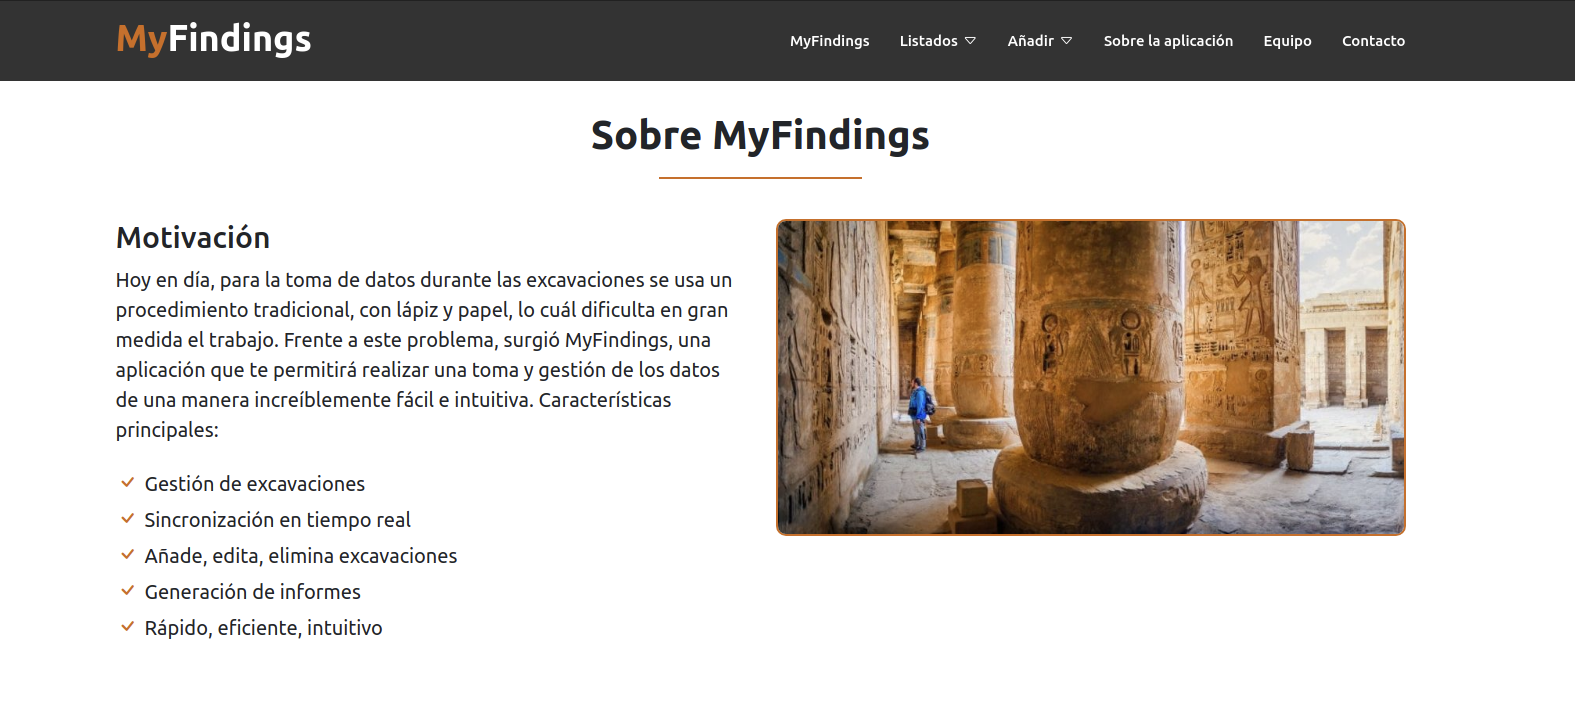
\includegraphics[scale=0.20]{imagenes/about.png}
            \caption[Sobre la aplicación]{Sobre la aplicación. Fuente \cite{petra-ad-deir}}
            \label{fig:about}
        \end{figure}

    Como puede observarse, el contenido principal de la página está dividido en dos filas
    o \textbf{rows} (normalmente se usa la terminología inglesa), la primera, que se
    corresponde con el título o \textbf{headline} (común en muchas páginas) y la segunda,
    que está dividida en dos partes que usan 6 columnas de Bootstrap cada una, conteniendo
    la \textbf{motivación} y la \textbf{imagen} respectivamente.

    \subsubsection{Equipo}
    Esta página contiene información sobre los componentes que hemos hecho posible este
    proyecto, en este caso, \textit{Joaquín García Venegas} y yo, \textit{Joaquín
    Alejandro España Sánchez}\\
    
    Por supuesto, ambos hacemos funciones totalmente distintas, por un lado la aplicación
    android y por otro la aplicación web, sobre lo que nos centraremos en este proyecto.
    Ambos componentes son diferentes, pero en su conjunto forman \textbf{MyFindings},
    un proyecto completamente funcional. La página quedaría tal que así:

        \begin{figure}[H]
            \centering
            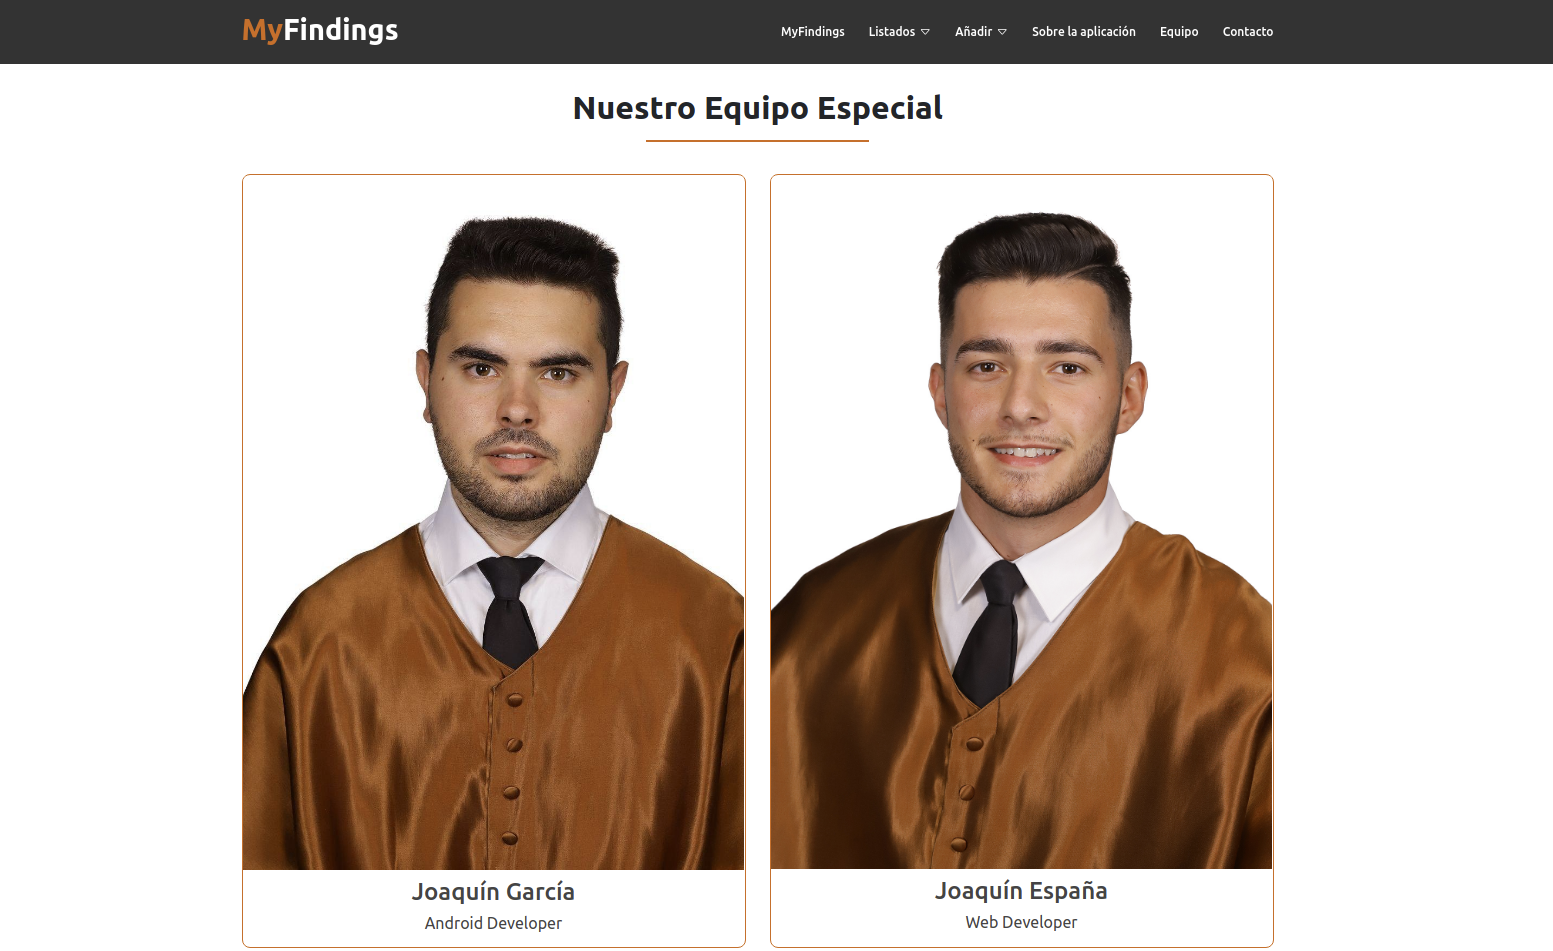
\includegraphics[scale=0.25]{imagenes/team.png}
            \caption{Equipo de MyFindings}
            \label{fig:team}
        \end{figure}

    En este caso se ha utilizado una estructura de página muy parecida a la anterior, utilizando
    dos rows, el primero para el \textbf{headline} y el segundo para los \textbf{miembros} del
    proyecto. Cabe mencionar el uso de la clase \textbf{border-box} en numerosas ocasiones en 
    el código, éste incorpora un border naranja al componente que lo posea.

    \subsubsection{Contacto}
    Finalmente, tenemos la página de contacto de la aplicación web, en ella podemos
    encontrar datos como el correo electrónico del desarrollador y su página de
    \href{https://github.com/alexespana/}{Github} o un mapa del lugar de residencia del
    programador, en este caso Granada.\\

        \begin{figure}[H]
            \centering
            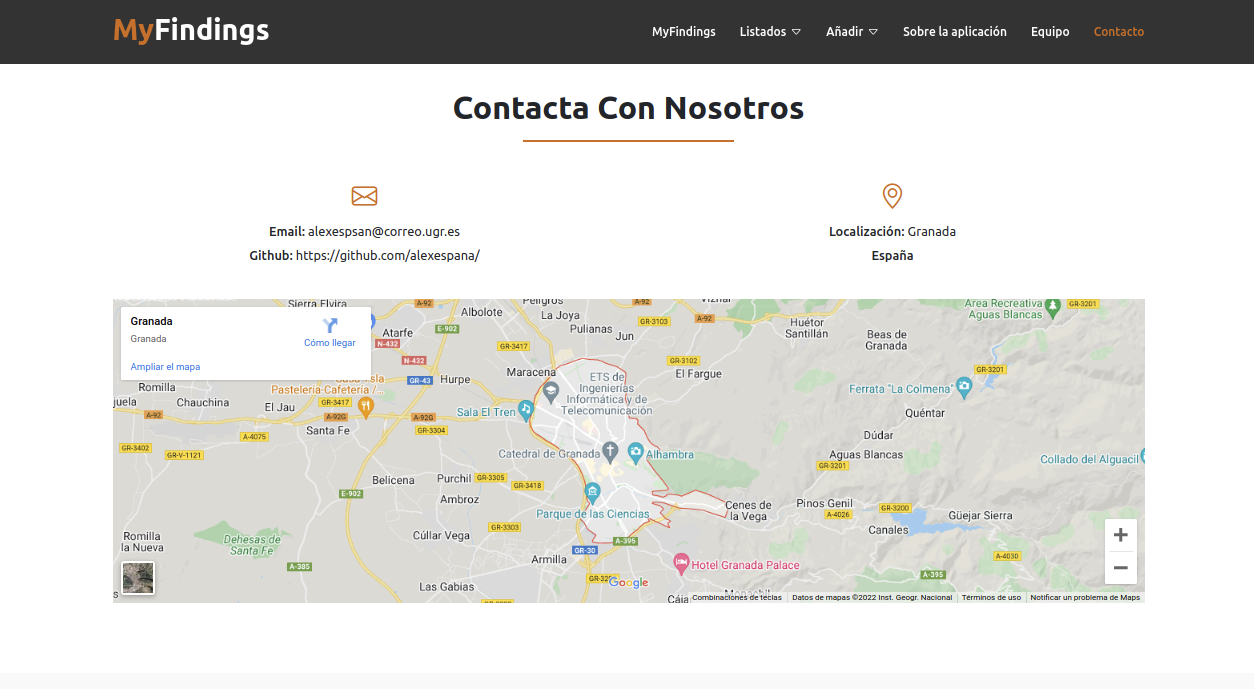
\includegraphics[scale=0.20]{imagenes/contact.png}
            \caption{Contacto de MyFindings}
            \label{fig:contact}
        \end{figure}

    Para realizar esta página se ha hecho uso de tres filas, la primera de ellas
    está destinada al \textbf{headline}, que como hemos visto, es común en otras páginas, 
    por lo que usan la misma clase de estilo CSS. La segunda a su vez está dividida en 
    dos partes utilizando cada una 6 columnas y finalmente la tercera fila ha sido
    destinada para el \textbf{iframe} de google maps cuyo código html ha sido extraído
    directamente de la aplicación web y puesto sobre el código.

\subsection{Creación de la base de datos}
Este milestone es uno de los más importantes del proyecto ya que tiene como principal objetivo
la definición de la base de datos que se utilizará, que posteriormente nos permitirá hacer las
consultas apropiadas según las necesidades que busca el cliente, en este caso los arqueólogos.\\

No prestarle atención a este hito sería un grave error, ya que si se realiza un mal diseño
de la BD puede conducir a las siguientes consecuencias en el desarrollo de software:

    \begin{itemize}
        \item El proyecto podría \textbf{fallar} al no soportar los requerimientos de la
        aplicación.
        \item Si hay un diseño muy complejo, el costo de desarrollo se verá
        \textbf{incrementado} ya que habrá que implementar más código para solucionar las
        distintas dificultades de la DB.
        \item Una base de datos compleja puede tener \textbf{gran cantidad de tablas} que 
        provocan código innecesario y complejo de entender.
        \item Posibles relaciones erróneas entre los datos que pueden llegar a provocar
        \textbf{fallos en la actualización} de los mismos y que finalmente sea necesario realizar
        actualizaciones manuales.
    \end{itemize}

En este caso, necesitamos utilizar una \textbf{base de datos relacional} ya que gran número
de tablas están relacionadas entre sí, existiendo claves externas e incluso claves
candidatas que se forman a partir de claves primarias y atributos discriminadores de
relaciones. Todo esto, se verá en la sección siguiente.

    \subsubsection{Modelo E/R}
    El modelo E/R es la técnica de modelado de datos más extendida para el diseño
    conceptual ya que posee una gran capacidad expresiva (a simple vista se pueden
    distinguir las distintas entidades con sus atributos y relaciones), es rigurosa, simple
    y fácil de emplear. Nos permite especificar las necesidades de información de nuestro
    proyecto permitiéndonos hacer un diseño \textbf{\textit{apropiado}},
    \textbf{\textit{de calidad}} y \textbf{\textit{fácil de transmitir}}.\\

    Para realizar dicho diseño, se ha hecho conjuntamente con \textit{Joaquín García 
    Venegas}, ya que para la aplicación android también será necesario tener el diseño de la
    BD. Este modelo deberá:

        \begin{enumerate}
            \item Reflejar fielmente las necesidades de información del proyecto. Ésto permite
            partir de una base para el desarrollo del sistema.
            \item Ofrecer un diseño independiente a la forma en que los datos serán
            posteriormente almacenados y sus formas de acceso, permitiendo tomar decisiones
            objetivas sobre la implementación más idónea.
        \end{enumerate}

    Teniendo todo esto en cuenta, el modelo E/R resultante para nuestro proyecto es el
    siguiente (si por cuestiones de editor o de pantalla no se puede ver correctamente,
    ir al siguiente enlace 
    \url{https://drive.google.com/file/d/1CRU5W9OQKCQF8nEYkDnl53O0noaJ9DS6/view?usp=sharing}):

        \begin{figure}[H]
            \centering
            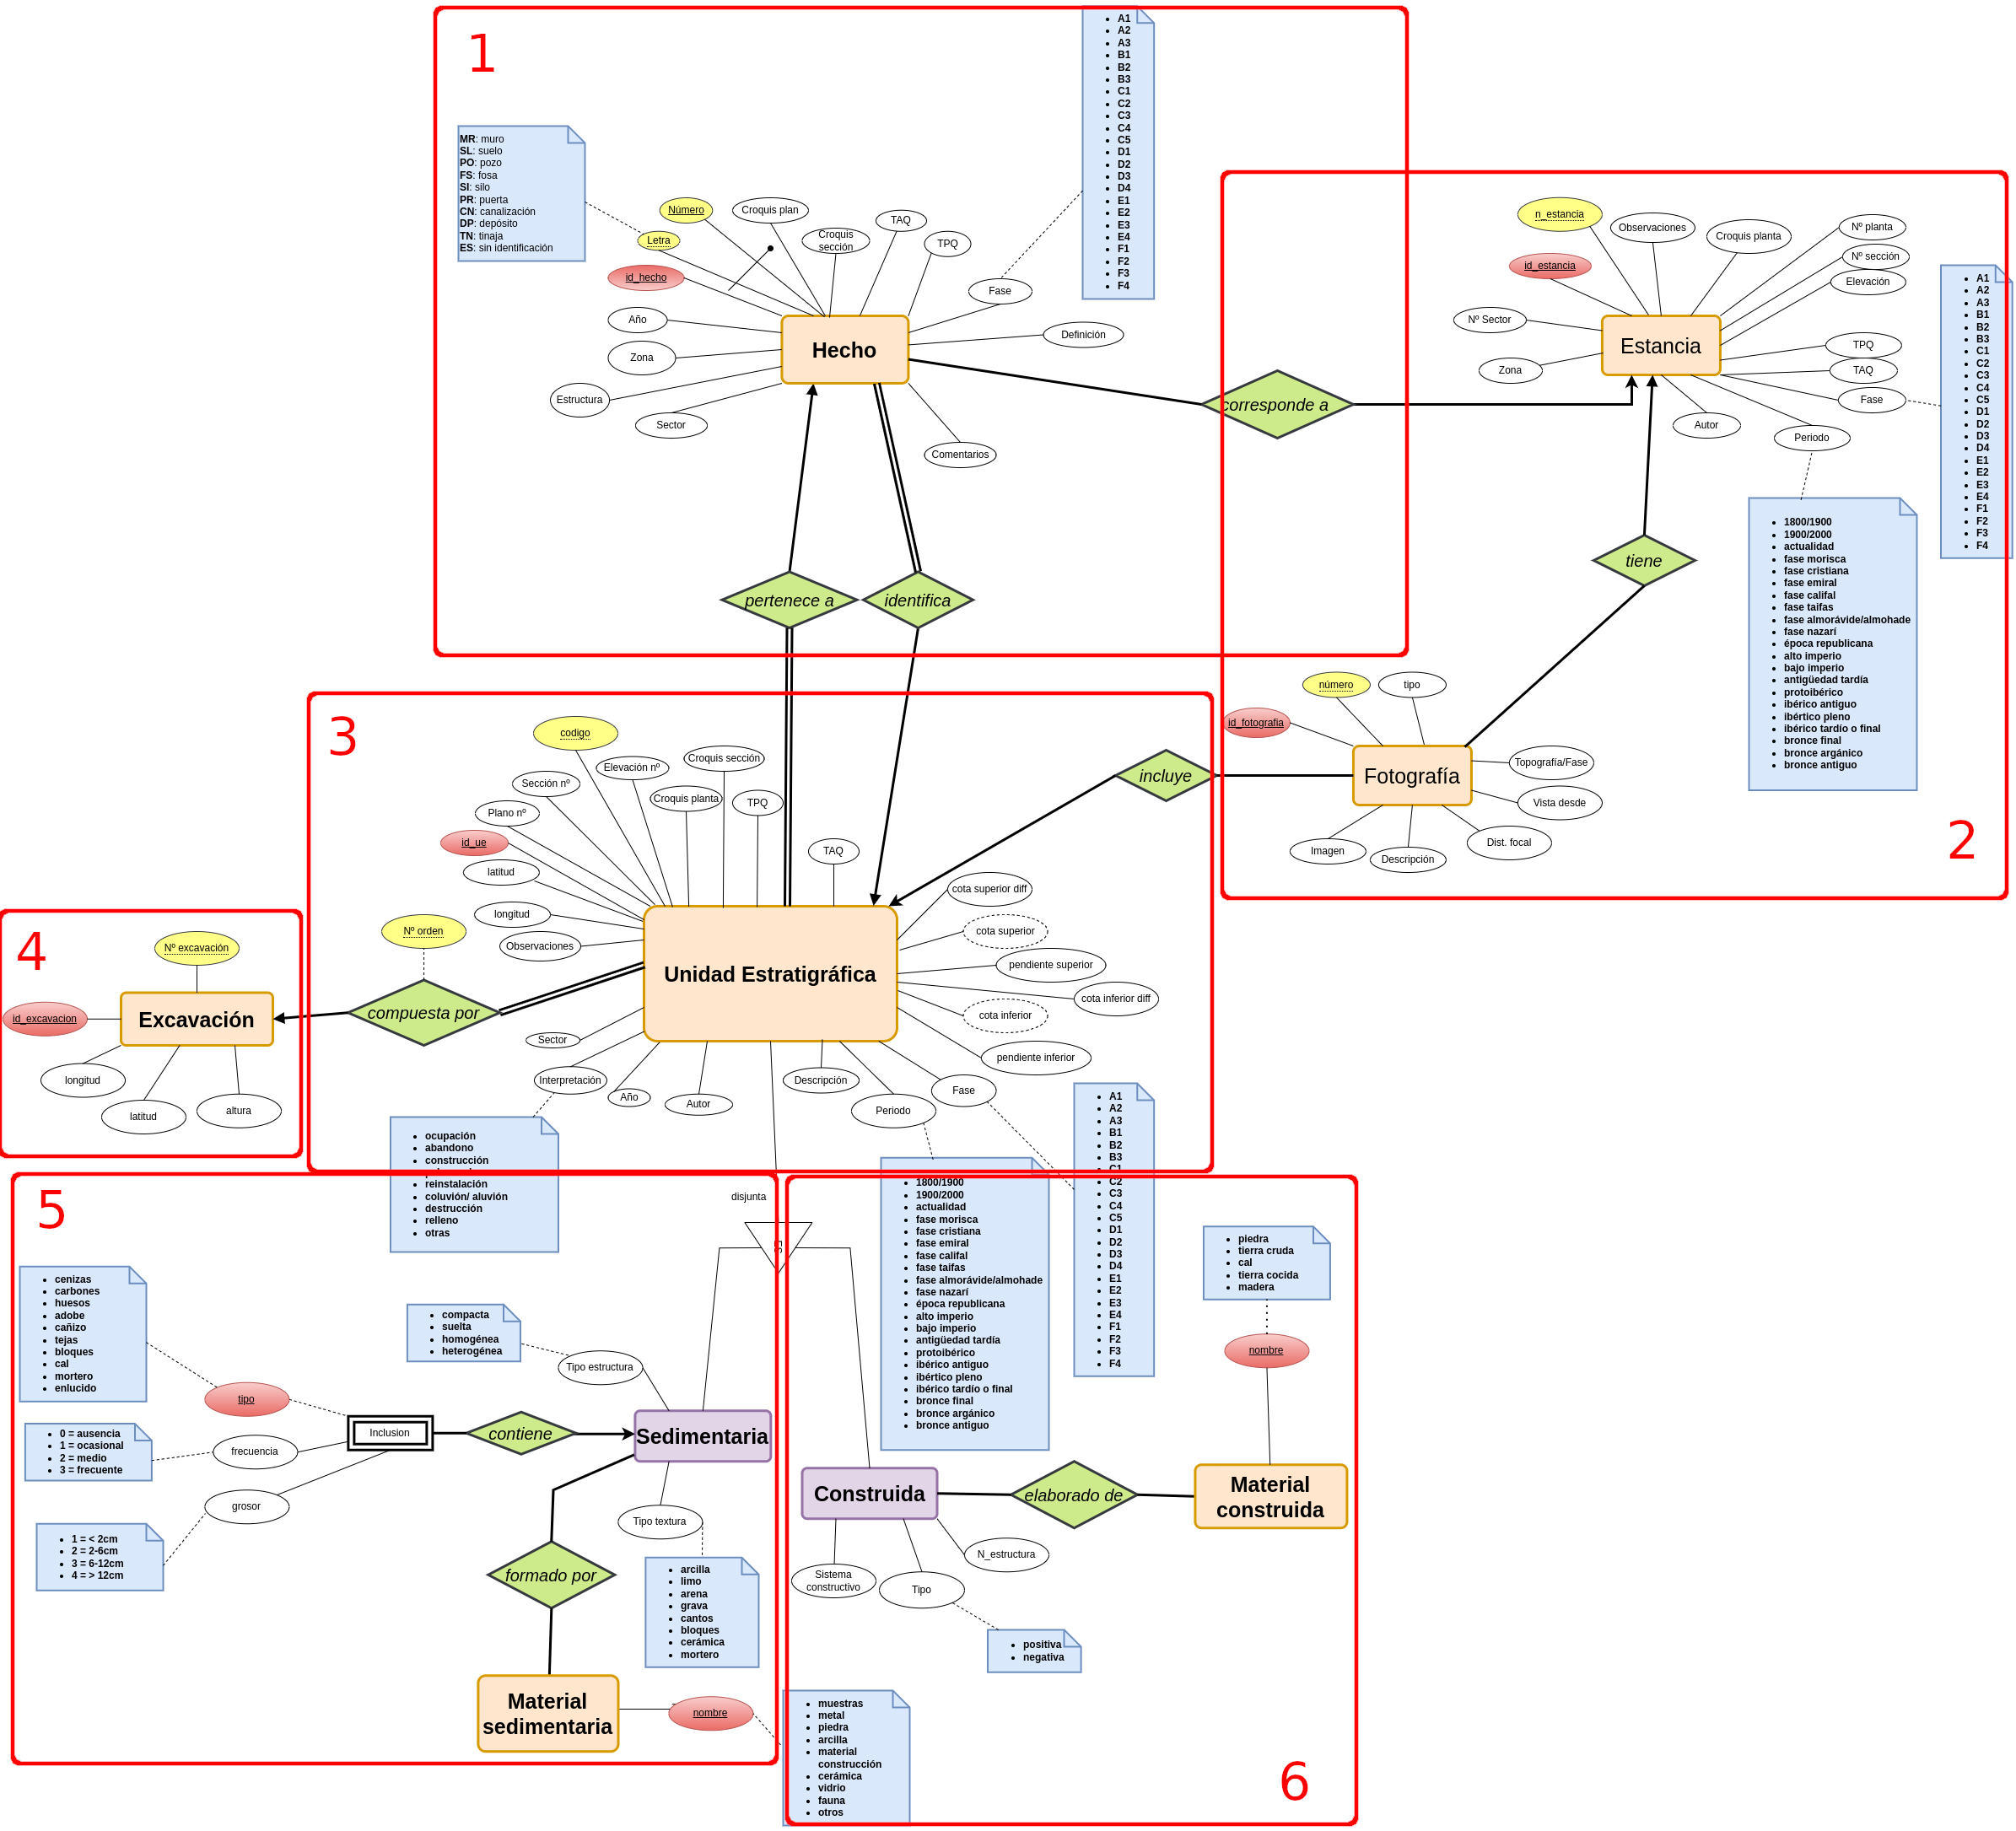
\includegraphics[scale=0.15]{imagenes/E-RModel.png}
            \caption{Modelo Entidad/Relación}
            \label{fig:e-rmodel}
        \end{figure}

    Por cuestiones de comodidad, se ha dividido la imagen en secciones que se pueden ver
    ampliadas en las páginas siguientes. Si se desea ir directamente a una sección, pulse
    sobre la sección deseada: sección 1 (\textbf{\ref{fig:e-rmodel1}}), sección 2
    (\textbf{\ref{fig:e-rmodel2}}), sección 3 (\textbf{\ref{fig:e-rmodel3}}), sección 4
    (\textbf{\ref{fig:e-rmodel4}}), sección 5 (\textbf{\ref{fig:e-rmodel5}}) y sección 6
    (\textbf{\ref{fig:e-rmodel6}}).

        \begin{figure}[H]
            \centering
            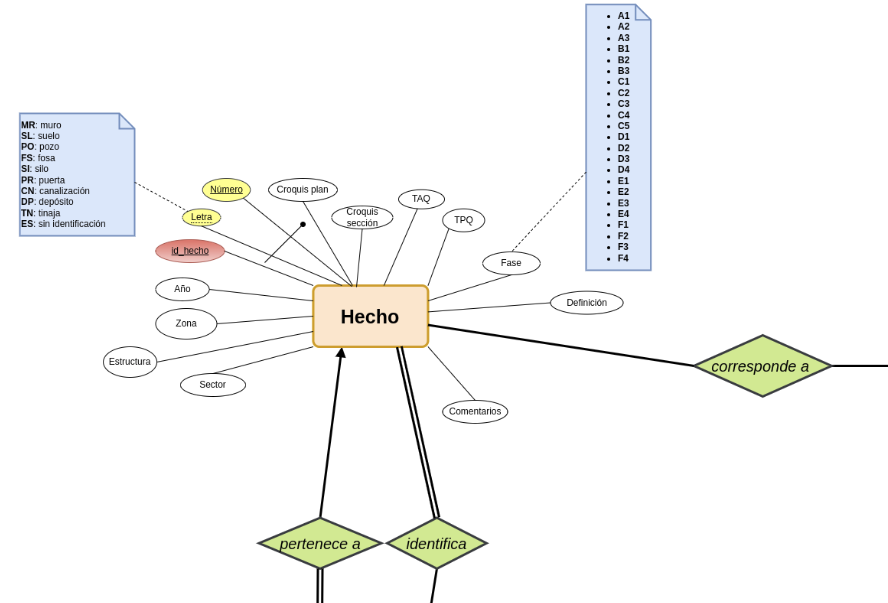
\includegraphics[scale=0.40]{imagenes/E-R1.png}
            \caption{Modelo E/R: sección 1}
            \label{fig:e-rmodel1}
        \end{figure}

        \begin{figure}[H]
            \centering
            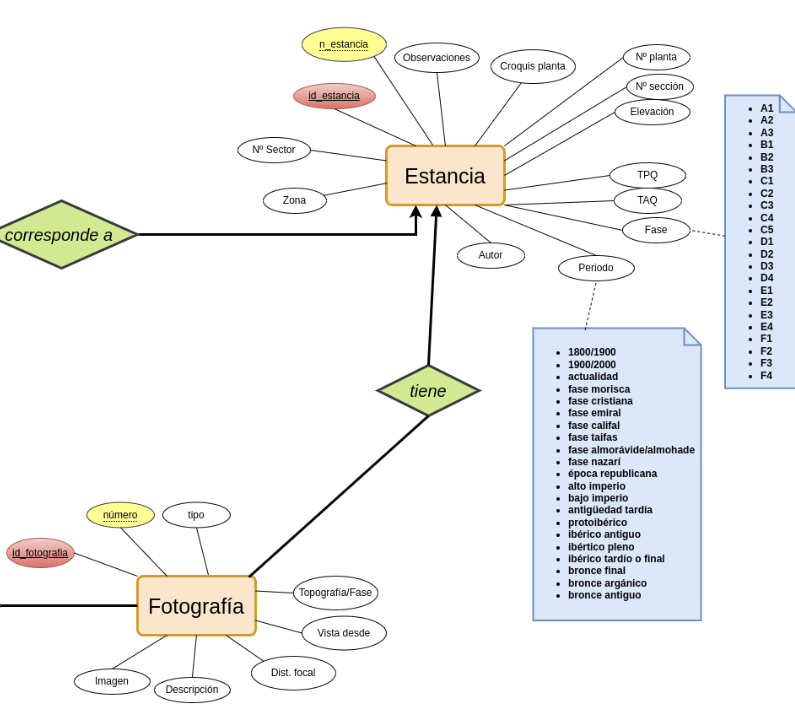
\includegraphics[scale=0.40]{imagenes/E-R2.png}
            \caption{Modelo E/R: sección 2}
            \label{fig:e-rmodel2}
        \end{figure}

        \begin{figure}[H]
            \centering
            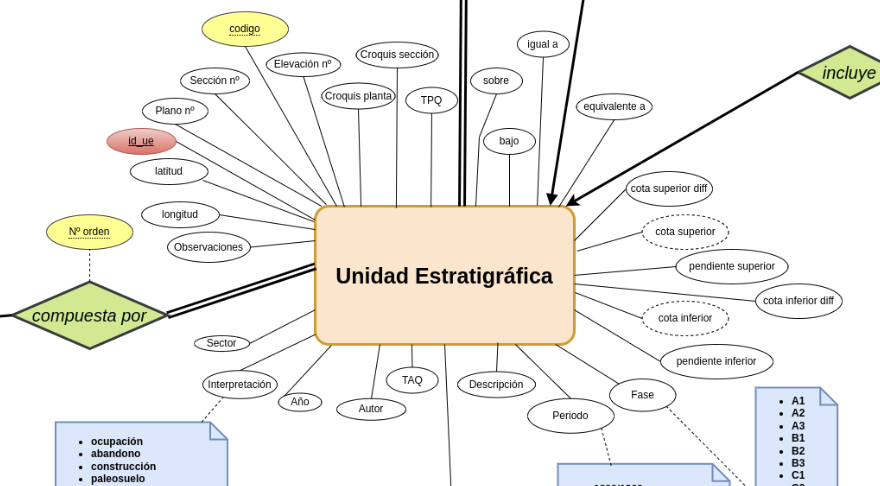
\includegraphics[scale=0.32]{imagenes/E-R3.png}
            \caption{Modelo E/R: sección 3}
            \label{fig:e-rmodel3}
        \end{figure}

        \begin{figure}[H]
            \centering
            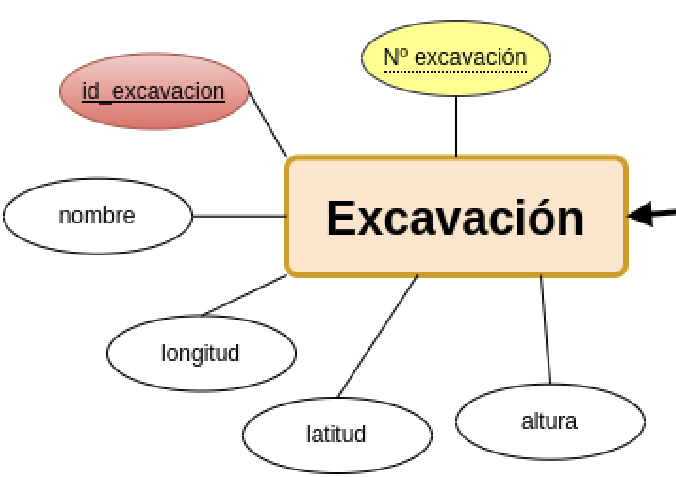
\includegraphics{imagenes/E-R4.png}
            \caption{Modelo E/R: sección 4}
            \label{fig:e-rmodel4}
        \end{figure}

        \begin{figure}[H]
            \centering
            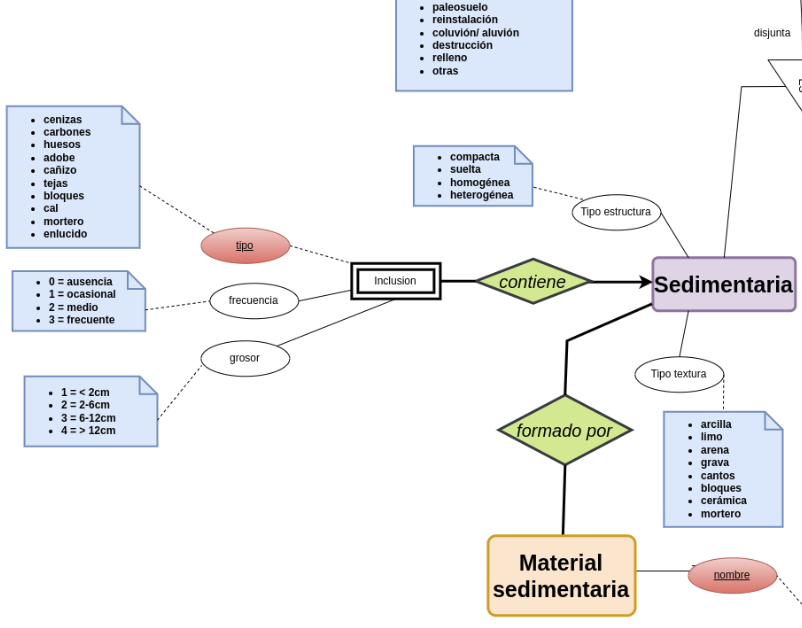
\includegraphics[scale=0.35]{imagenes/E-R5.png}
            \caption{Modelo E/R: sección 5}
            \label{fig:e-rmodel5}
        \end{figure}

        \begin{figure}[H]
            \centering
            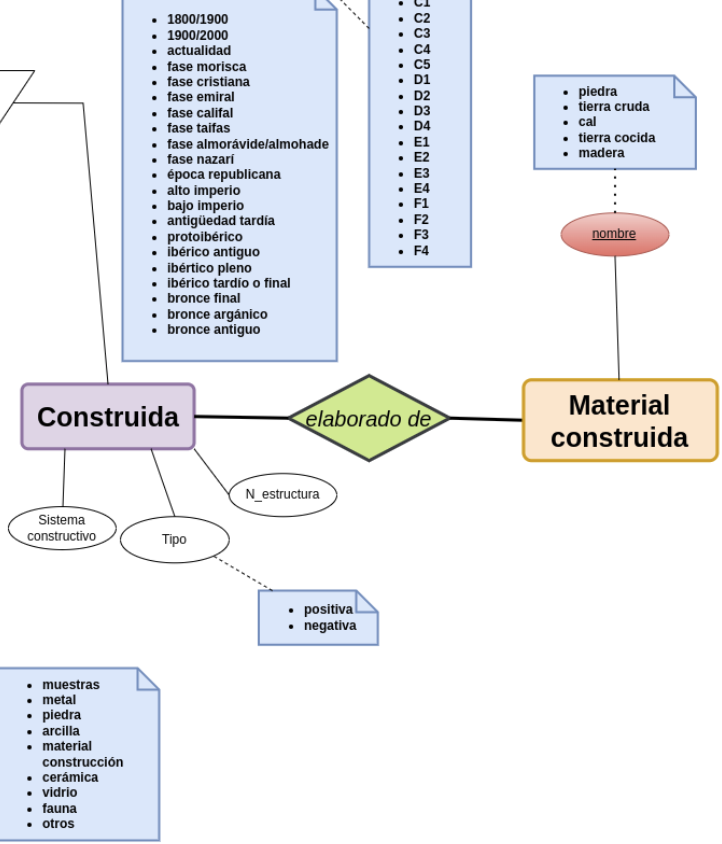
\includegraphics[scale=0.35]{imagenes/E-R6.png}
            \caption{Modelo E/R: sección 6}
            \label{fig:e-rmodel6}
        \end{figure}


    Vamos a comenzar justificando las elecciones más importantes que se han ido tomando
    sobre el modelo, para ello seguiré el siguiente orden: \textbf{entidades fuertes},
    \textbf{herencia}, \textbf{entidades débiles} y \textbf{relaciones}.\\

    \subsubsection{Entidades fuertes}
    Como podemos observar, hay siete entidades fuertes, entre las que podemos destacar,
    además de los atributos necesarios que no son claves primarias o candidatas, lo siguiente:

    \begin{enumerate}
        \item \textbf{Excavación}: ésta tendrá un identificador interno en la base de
        datos que actuará como primary key, que será un valor numérico, y además una clave
        candidata que será el \textbf{número de excavación}, un entero de tres dígitos
        (p.ej: 001, 043, 132, etc). Esta clave candidata será la visible al usuario, pudiendo
        introducir el número de excavación deseado.

        \item \textbf{Unidad Estratigráfica}: al igual que la anterior, tendremos un
        identificador interno que será la primary key, y además, una clave candidata que
        será el \textbf{código} de la unidad estratigráfica, que servirá para que el usuario
        pueda identificar dicha unidad. Dicho código debe estar formado por el
        \textbf{número de excavación} al que pertenece la unidad más el \textbf{número de orden}
        de la unidad en la excavación. Por ejemplo, si la unidad pertenece a la excavación
        \textbf{001} y es la unidad número 32 encontrada en la excavación (\textbf{032}), el
        código que identificaría a la unidad sería el \textbf{001032}.

        \item \textbf{Hecho}: la forma que tiene el usuario de identificar a cada hecho es algo
        más compleja. Al igual que las dos entidades anteriores, también se tendrá un
        identificador interno que actuará de primary key, y además, se tendrá una clave
        candidata compuesta, que estará formada por la \textbf{letra} (tipo de hecho) y un
        \textbf{número}. Para poder darle un valor coherente a este número, se elige una
        unidad estratigráfica perteneciente al hecho y el código de dicha unidad será el
        número(\textbf{parte de la clave candidata}) de dicho hecho. Por ejemplo, si tenemos
        la unidad estratigráfica con código \textbf{001032} y dicha unidad es la que sirve
        para identificar al hecho de tipo muro (\textbf{MR}) la clave candidata del hecho
        sería \textbf{MR001032}.

        \item \textbf{Estancia}: en este caso, al igual que las entidades anteriores,
        tendremos un identificador interno como primary key que solo se conocerá internamente
        en el sistema, y además, tendremos un \textbf{número de estancia}, que será la clave
        candidata de la entidad, visible y reconocible para los usuarios de la aplicación. Al
        comienzo del diseño pensábamos que el número de estancia se formaba a partir del número
        de sector y el número de zona, como está reflejado en el anexo \ref{subsec: doubts},
        pero finalmente éste esta formado por las letras ES seguidas de tres dígitos. Por ejemplo
        un posible identificador de estancia podría ser \textbf{ES001}.

        \item \textbf{Fotografía}: poseeremos un primary key interno para la entidad y una
        clave candidata que será el \textbf{número} de la fotografía. Las fotografías están
        relacionadas tanto con las unidades estratigráficas como con las estancias, y es que 
        ambas pueden tener fotografías concretas.
        
        \item \textbf{Material construido}: esta entidad surge porque una unidad estratigráfica
        construida puede estar construida con \textbf{varios tipos de materiales} construidos,
        de ahí el hecho de que no se pueda poner simplemente un atributo que sea material en
        la unidad construida y se tenga que añadir una nueva entidad.

        Al comienzo podría pensarse que el material es una entidad débil de la unidad
        construida, pero esto traería problemas ya que para identificar a un material sería
        necesario el identificador de la unidad estratigráfica y el atributo discriminador de
        la entidad débil. Esto carecería de sentido ya que podría haber dos UE's construidas
        con el mismo material, pero cada uno se identificaría de una forma distinta, a pesar
        de ser el mismo material. Por esta razón se consideró como una entidad fuerte, a la
        que muchas unidades estratigráficas construidas pueden estar asociadas. Tiendo esto
        en cuenta, esta vez no tendremos un primary key interno, sino que el \textbf{nombre}
        del material será la primary key. Por ejemplo: el material \textbf{Piedra} pudiese
        formar parte de 50 unidades construidas, siendo únicamente necesario el 
        \textbf{nombre} del material para identificar a uno.
        
        \item \textbf{Material sedimentario}: esta entidad, al igual que la anterior, surge
        porque una unidad estratigráfica sedimentaria puede estar construida con 
        \textbf{varios tipos de materiales} sedimentarios, de ahí el hecho de que no se pueda
        poner simplemente un atributo que sea material en la unidad sedimentaria y se tenga que
        añadir una nueva entidad.

        En este caso también podríamos pensar que el material es una entidad débil de la unidad
        sedimentaria, pero esto también traería problemas ya que para identificar a un material
        sería necesario el identificador de la unidad sedimentaria y el atributo discriminador
        de la entidad débil, que en este caso sería el \textbf{nombre}. Como hemos mencionado
        anteriormente, no tiene sentido ya que podría haber dos UE's sedimentarias hechas
        con el mismo material, pero cada uno se identificaría de una forma distinta, a pesar
        de ser el mismo material. Por esta razón se consideró como una entidad fuerte, a la
        que muchas unidades estratigráficas sedimentarias pueden estar asociadas. Igual que el
        anterior, la primary key sería el \textbf{nombre} del material. Por ejemplo: el
        material \textbf{Metal} pudiese formar parte de 10 unidades sedimentarias, siendo
        únicamente necesario el \textbf{nombre} del material para identificar a uno. 
    \end{enumerate}

    \subsubsection{Herencia}
    Como podemos comprobar en el modelo E/R, existen claramente dos entidades que heredan de
    la entidad fuerte Unidad Estratigráfica, la \textbf{Sedimentaria} y la \textbf{Construida}.
    Ambas heredarán todos los atributos de la entidad padre y además añadirán sus propios
    atributos. En las fichas de registro de campo completo \ref{sec:registrationforms} puede
    verse en la UE construida como existe un apartado material, sin embargo, en la sedimentaria
    no existe una sección como tal, la pregunta sería: \textbf{¿por qué las UE sedimentarias
    tienen un material distinto entonces?} Tras numerosas entrevistas con el arqueólogo al
    final se dedujo que los materiales de la primera hoja de \ref{sec:registrationforms}
    correspondian a materiales que sólo las UE's sedimentarias podían tener, por esta razón
    se incorporaron.

    \subsubsection{Entidades débiles}
    La única entidad débil del modelo E/R es la \textbf{Inclusión}. Dicha entidad surge porque
    una inclusión posee distintos atributos como la \textbf{frecuencia}, el \textbf{grosor} y
    el \textbf{tipo}, por lo que habría que modelarlos como una entidad que recogiese todos
    estos datos, además de que una unidad sedimentaria podría tener varias de ellas. En este
    caso, sí tiene sentido reflejarla como una \textbf{entidad débil} ya que las inclusiones
    son propias de cada UE y no se comparten con otras unidades sedimentarias.\\

    Por lo tanto, estaría identificada por el \textbf{identificador} de la unidad estratigráfica
    sedimentaria y el atributo discriminador de la entidad débil que en este caso es el
    \textbf{tipo} (que puede ser cenizas, carbones, huesos, adobe, etc).

    \subsubsection{Relaciones}
    Finalizando con las relaciones, voy a enumerar las distintas relaciones identificando las
    entidades implicadas:

        \begin{enumerate}
            \item \textbf{Compuesta por (Excavación-UE)}: relación uno a muchos (1:M). En la
            relación se guarda el número de orden de la unidad estratigráfica.
            \item \textbf{Pertenece a (UE-Hecho)}: relación muchos a uno (M:1).
            \item \textbf{Identifica (UE-Hecho)}: relación uno a muchos (1:M).
            \item \textbf{Corresponde a (Hecho-Estancia)}: relación muchos a 1 (M:1).
            \item \textbf{Tiene (Estancia-Fotografía)}: relación uno a muchos (1:M).
            \item \textbf{Incluye (Fotografía-UE)}: relación muchos a uno (M:1).
            \item \textbf{Contiene (Sedimentaria-Inclusión)}: relación 1 a muchos (1:M).
            \item \textbf{Formado por (Sedimentaria-Material sedimentaria)}: relación muchos a
            muchos (M:N).
            \item \textbf{Elaborado de (Construida-Material construida)}: relación muchos a
            muchos (M:N).
        \end{enumerate}

    \subsubsection{Django ORM}

    Ahora vamos a hablar un poco sobre la implementación \textbf{en el código}, en la forma
    de representar el modelo E/R en nuestra aplicación \textbf{Django}.\\

    \paragraph{¿Qué es un ORM?} \underline{}                                            
    \newline Antes de nada, vamos a explicar qué es un \textbf{ORM (Object Relational Mapping)}, ya
    que será un concepto clave para entender lo posteriormente explicado. Un ORM es un modelo
    de programación que nos permite mapear las estructuras de una base de datos relacional
    sobre unas estructuras lógicas en el código (por ejemplo objetos), es decir, nos permite
    convertir los objetos de nuestra aplicación en un formato adecuado (SQL) para ser
    almacenado en la base de datos. Como todo en la vida, esto tiene unas ventajas y unas
    desventajas, comencemos por las ventajas:

        \begin{enumerate}
            \item Hacen que el proceso de desarrollo sea más rápido.
            \item No se necesita tener \textbf{conocimiento de SQL } para usar el ORM. Esto
            hace que la complejidad del DML se reduciese, evitando tener que hacer joins,
            multi-inserciones, sub-selecciones, etc.
            \item El ORM asegura la consulta para cualquier tipo de ataque.
        \end{enumerate}

    A pesar de tener cosas muy buenas, el ORM también tiene algunos aspectos que podrían
    considerarse pequeñas desventajas:

        \begin{enumerate}
            \item Los ORMS generan una consulta y la pasan a la base de datos. En ocasiones
            estas consultas devuelven una matriz con un formato complejo con
            \textbf{colecciones}(objetos) que tienen información no relevante para nosotros
            \item Cuando la lógica de negocio de la aplicación se vuelve compleja, a veces
            no se puede representar mediante un ORM, aunque sí pueda ser manejable a nivel
            de consulta
        \end{enumerate}

    Dicho todo esto, podemos comenzar a hablar sobre el ORM que utilizaremos para la
    aplicación web, el \textbf{ORM de Django}. Éste nos permite diseñar nuestras tablas de 
    base de datos sin necesidad de escribir ninguna sentencia SQL, en este caso, en
    \textbf{PostgreSQL}. Un modelo es la fuente de información única y definitiva para los
    datos, éste contendrá los campos y funcionalidades(comportamiento) correspondientes a
    la naturaleza de los datos que almacena. Normalmente, cada modelo se asigna a una sola
    tabla de base de datos, y cada uno de ellos:

        \begin{itemize}
            \item Es una clase de python que hereda de la clase \textbf{django.db.models.Model}.
            \item Cada atributo de la clase representa un campo (columna) de la base de datos.
            \item Al corresponderse cada entidad a una clase, Django proporciona automáticamente
            una \textbf{API de abstracción de bases de datos} que nos permite realizar las
            operaciones de \textbf{CRUD} básicas: crear, recuperar, actualizar y eliminar
            objetos.
        \end{itemize}

    Cada modelo visible para el usuario tiene una función \textbf{\textit{str}} que se
    corresponde con la identificación del objeto al mostrarlo al usuario. Digamos que se
    trata de un método especial que devuelve una representación en forma de \textbf{string} de
    cualquier objeto y que Python y Django utilizarán cada vez que una instancia de un 
    modelo necesite ser mostrada como una cadena, como puede ser en el caso de la consola
    interactiva, en la vista de administrador, en un display de una tabla, etc.\\

    Pongamos un ejemplo, si la unidad estratigráfica posee un \textbf{ForeignKey} que es
    la \textbf{excavación} a la que pertenece, dicha instancia de excavación se mostraría
    para el usuario como el \textbf{número de excavación}, ya que en el modelo de la
    excavación existirá un método str que devolvería el \textbf{n\_excavacion},
    quedando el modelo de la siguiente forma:

    % % DESCOMENTAR
    % \begin{minted}[mathescape, linenos,numbersep=5pt,bgcolor=lightgray,gobble=2,
    %                frame=lines,fontsize=\footnotesize,framesep=2mm]{python}
    % class Excavacion(models.Model):
    %     n_excavacion = models.PositiveIntegerField(unique=True, 
    %                     verbose_name='Número de excavación')
    %     latitud = models.FloatField()
    %     longitud = models.FloatField()
    %     altura = models.PositiveSmallIntegerField()

    %     def __str__(self):
    %         return str(self.n_excavacion)
    % \end{minted}

    Si nos fijamos, vemos que es necesario que esta función devuelva un string, por esta
    razón se usa la función str en el return. Además, Django nos proporciona \textbf{gran
    variedad de tipos posibles} para los campos de los modelos, por lo que nos podemos
    ahorrar hacer algunas comprobaciones en los formularios de recogida de datos, aunque
    algunas serán necesariamente obligatorias. Aquellos campos que necesiten ser positivos
    utilizarán campos de tipo \textbf{PositiveSmallIntegerField}, que nos permite introducir
    enteros desde el 0 hasta el 32767, cantidades suficientes para el contexto de nuestro
    proyecto.\\

    Lo siguiente va a ser explicar cómo representar en los modelos las \textbf{primary keys},
    \textbf{candidate keys} y \textbf{relationships}.\\
    
    \paragraph{Claves primarias} \underline{}
    \newline En los atributos de los modelos, en los tipos de campo, existe un parámetro llamado
    \textbf{primary\underline{ }key}, si se indica a True, entonces dicho campo será la clave
    primaria del modelo, pero si no se indica el primary key en ningún campo del modelo,
    entonces django automáticamente añadirá un campo \textbf{id} para guardar la clave primaria.
    Dicho atributo será un campo de tipo \textbf{models.BigAutoField}, que nos permite números
    desde el 1 hasta el 9223372036854775807, por lo que no habrá ningún tipo de problema con
    la generación de los id's. Por supuesto, si en algún campo se declara \textbf{explícitamente}
    la clave primaria, django no generará el campo id y el campo que hayamos elegido pasará a
    ser clave primaria. En nuestro modelo E/R, las claves primarias que se generarán
    automáticamente por django en los modelos serán las de \textbf{Excavacion, UE, Hecho,
    Estancia y Fotografia}. 
    
    \paragraph{Claves candidatas} \underline{}
    \newline Para las \textbf{claves candidatas simples} únicamente hay que indicar en el campo
    correspondiente al argumento \textbf{unique} a True. Por ejemplo, en el modelo
    \textbf{Excavación} mostrado anteriormente el campo del número de excavación es
    candidate key:
    
    % % DESCOMENTAR
    % \begin{minted}[mathescape, linenos,numbersep=5pt,bgcolor=lightgray,gobble=2,
    %                frame=lines,fontsize=\footnotesize,framesep=2mm]{python}
    % class Excavacion(models.Model):
    %     n_excavacion = models.PositiveIntegerField(unique=True, 
    %                     verbose_name='Número de excavación')
    %     .
    %     .
    % \end{minted}

    ¿Cómo se representaría una clave candidata compuesta? En Django, esto se puede hacer de
    dos formas posibles:

    \begin{enumerate}
        \item Mediante la opción \textbf{unique\underline{ }together}, que incluye la lista
        de campos que formarán la clave candidata, y que por lo tanto conjuntamente serán
        únicos. Vamos a hacer el ejemplo con el modelo Hecho, ya que es el único que tiene
        una clave candidata compuesta:
        
    % % DESCOMENTAR
    % \begin{minted}[linenos,numbersep=5pt,bgcolor=lightgray,gobble=2,
    %     frame=lines,fontsize=\footnotesize,framesep=2mm]{python}
    % class Excavacion(models.Model):
    %     letra = models.CharField(max_length=2, choices=LETRA_CHOICES)
    %     numero = models.CharField(max_length=6)    
    %     .
    %     .
    %     class Meta:
    %         unique_together = ('letra', 'numero',)
    % \end{minted}

        \item La forma anterior, sin embargo, no es del todo aconsejable por django ya
        que sugiere utilizar \textbf{UniqueConstraint} con la opción \textbf{constraint},
        ya que la opción de \verb|unique_together| ofrece menor funcionalidad y puede
        estar deprecated en un futuro. Con esta nueva forma, la clase de metadatos
        del modelo quedaría así:
        
    % % DESCOMENTAR
    % \begin{minted}[linenos,numbersep=5pt,bgcolor=lightgray,gobble=2,
    %     frame=lines,fontsize=\footnotesize,framesep=2mm]{python}
    % class Excavacion(models.Model):
    %     letra = models.CharField(max_length=2, choices=LETRA_CHOICES)
    %     numero = models.CharField(max_length=6)    
    %     .
    %     .
    %     class Meta:
    %         constraints = [
    %             models.UniqueConstraint(fields=['letra', 'numero'], 
    %                                     name='fact_constraint')                                                  
    %         ]
    % \end{minted}

    Dicha restricción tendrá el nombre de \textbf{fact\underline{ }constraint}.
    \end{enumerate}

    \paragraph{Relaciones} \underline{}
    \newline Django soporta las mismas tres relaciones que existen en una base de datos relacional:
    uno a uno, uno a muchos, y muchos a muchos. Para representarlas, usa tres tipos de campos
    para los modelos, que son:

        \begin{itemize}
            \item \textbf{OneToOneField}: en uno de los modelos implicados, recibe como
            argumentos básicos el nombre del modelo con el que está asociado y el argumento
            del borrado en cascada (\textbf{on\underline{ }delete}).
            \item \textbf{ForeignKey}: en el modelo de la parte \textbf{muchos}, irá un campo
            con el nombre del modelo asociado en minúscula y de tipo ForeignKey, recibiendo
            como parámetros el nombre del modelo asociado (parte del uno) y el argumento del
            borrado en cascada.
            \item \textbf{ManyToManyField}: este tipo de relaciones son algo más complejas. Al
            ser una relación M:N podemos pensar que en cada uno de los modelos irá un campo
            ManyToManyField, pero esto no es así. En el modelo donde tenga más lógica que vaya
            el campo muchos a muchos irá un campo con el nombre del otro modelo en plural (por
            \textbf{convención}) con el dato de tipo ManyToManyField, que recibe como parámetro
            únicamente el nombre del modelo con el que se relaciona.

            Por ejemplo, tengamos los modelos Pizza y Topping, ¿qué se entiende mejor?
            \textbf{¿que una pizza pueda tener muchos toppings?}, \textbf{¿o que un
            topping pueda estar en muchas pizzas?} La primera de las opciones es más
            intuitiva y por tanto el modelo Pizza tendría un campo toppings de tipo
            ManyToManyField.
        \end{itemize}

    Explicadas las formas de representar las relaciones en Django, voy a mencionar las
    relaciones que se dan en nuestro modelo:

        \begin{enumerate}
            \item El \textbf{Hecho} tiene una clave externa referenciando a la estancia a la
            que está asociado.
            \item La \textbf{UE}(unidad estratigráfica) tiene dos claves externas, una
            referenciando a la excavación con la que está asociada y otra referenciando al
            hecho al que pertenece.
            \item La \textbf{Fotografia} tiene también dos claves externas, una referenciando
            a la unidad estratigráfica asociada y otra referenciando a la estancia.
            \item La \textbf{Inclusion} tiene una clave externa referenciando la unidad
            estratigráfica sedimentaria a la que pertenece.
            \item La \textbf{UESedimentaria} tiene un campo ManyToManyField referenciando a
            los materiales sedimentarios (\textbf{MaterialSedimentaria}) por los que está
            formada.
            \item La \textbf{UEConstruida} tiene un campo ManyToManyField referenciando a
            los materiales construidos (\textbf{MaterialConstruida}) por los que está
            formada.
        \end{enumerate}

    Esta sería una visión global de la implementación utilizando el ORM que nos ofrece Django.

\subsection{Autenticación}
En este milestone del proyecto se ha trabajado sobre la autenticación y autorización de
usuarios en la aplicación web. A continuación se explicará todo lo que se ha
implementado.\\

Django cuenta con un \textbf{sistema de de autenticación} \cite{django-auth} de usuarios,
éste puede manejar cuentas de usuario, grupos de usuario, permisos, sesiones de usuario
basadas en cookies, etc. Antes de nada debemos de tener claro qué significan los términos
de autenticación y autorización:

    \begin{itemize}
        \item \textbf{Autenticación}: es un proceso en el que verifica que un usuario
        es quién dice ser. Por ejemplo, una de las pruebas más comunes de autenticación
        es mediante la escritura de una contraseña.
        \item \textbf{Autorización}: en este caso, se determina lo que un usuario
        autenticado puede hacer en el sistema, es decir, los permisos que éste posee. Por
        ejemplo, en nuestro caso, si puede o no modificar una excavación.
    \end{itemize}

Todo lo requerido para la autenticación en Django está implementado en uno de sus módulos,
concretamente en el módulo \textbf{django.contrib.auth}, que tendremos que añadirlo a
nuestro proyecto. Además, necesitaremos definir los permisos asociados a nuestros modelos,
por ejemplo, poder ver una excavacion, poder editarla, etc, para ello se usa el módulo
\textbf{django.contrib.contenttypes}, que también tendremos que añadir al proyecto.

\subsubsection{Vistas de autenticación}
En Django hay dos formas de implementar la autenticación de la aplicación: mediante la
definición de \textbf{tus propias vistas}, o utilizando las vistas \textbf{ya predefinidas}
de Django. En nuestro caso hemos obtado por la última, ya que nos ofrece todo lo necesario
para nuestro propósito y hace mucho más sencilla la implementación.\\

Para aclarar un poco más esto último, si nos fijamos en la figura \ref{fig:mvt}, lo que
estaríamos usando ya de forma predefinida por Django serían las urls (\textbf{URL}) y las
vistas (\textbf{VIEW}), quedando a nuestro cargo la definición de los correspondientes
\textbf{plantillas/templates} asociadas a cada una de las vistas y urls.\\

A continuación, se indican las rutas que se encuentran definidas en
\textbf{django.contrib.auth.urls} junto a la descripción de las funcionalidades de las
\textbf{plantillas/templates} que renderizan:

    \begin{itemize}
        \item \textbf{accounts/login/}: es el template desde el que los usuarios pueden
        loguearse en la aplicación, es decir, autenticarse.
        \item \textbf{accounts/logout/}: cuando un usuario está logueado y accede a esta
        url, se deslogueará automáticamente.
        \item \textbf{accounts/password\underline{ }change/}: permite a un usuario
        autenticado cambiar su contraseña en la aplicación.
        \item \textbf{accounts/password\underline{ }change/done/}: es el template que
        muestra el resultado del cambio de contraseña.
        \item \textbf{accounts/password\underline{ }reset/}: en caso de olvido de contraseña,
        este template permite a un usuario no logueado, introducir su correo para que se le
        envíe un enlace de recuperación de contraseña.
        \item \textbf{accounts/password\underline{ }reset/done/}: muestra el resultado de
        haber enviado el correo de recuperación de contraseña al usuario.
        \item \textbf{accounts/reset/<uidb64>/<token>/}: en este caso, la url anterior
        envía un enlace de recuperación de contraseña al usuario, este enlace tiene el
        formato aquí indicado, un \textbf{uidb64}, que sería el id del usuario codificado
        en base 64, y un \textbf{token}, que es un token de seguridad que se genera en
        el momento de la creación del enlace y verifica que el password sea válido.
        \item \textbf{accounts/reset/done/}: este template muestra un mensaje de confirmación
        tras el cambio de contraseña.
    \end{itemize}

\subsubsection{Registro de usuarios}
En este punto, dado que Django no ofrece ninguna vista ni url ya definida para el registro
de usuarios, se ha procedido a incorporar a nuestra aplicación una ruta (register/),
una vista (register) y una plantilla (register.html). Desde la plantilla, un usuario no
registrado en el sistema podrá registrarse introduciendo su \textbf{nombre de usuario}, un
\textbf{correo electrónico} (necesario para poder recuperar la contraseña en caso de
olvido), la \textbf{contraseña} y una \textbf{confirmación de contraseña}.\\

Para el registro de usuarios, se ha decidido que se siga el siguiente flujo de acciones en
la aplicación:

    \begin{enumerate}
        \item Un usuario no registrado rellena el formulario de registro y lo envía. Ahora
        estaría registrado en el sistema, pero como un usuario \textbf{inactivo}, por lo
        que no podrá loguearse en la aplicación.
        \item Al realizarse una solicitud de registro, se enviará un correo al administrador
        del sistema para que apruebe el registro del usuario.
        \item Al administrador del sistema aprueba el registro del usuario, \textbf{activando}
        al usuario desde su panel de administración.
        \item Se le notifica al usuario mediante correo electrónico que ya puede hacer login
        en la aplicación.
    \end{enumerate}

\subsubsection{Envío de correos}} 
El envío de correos electrónicos es una parte importante de la aplicación, ya que se
utiliza para enviar correos de recuperación de contraseña, para activar usuarios, para
confirmar las activaciones, etc.\\

A pesar de que python tiene una interfaz para enviar correos en el módulo de
\textbf{smtplib}, Django incorpora capas superiores para que el envío de los correos se
haga de forma mas rápida y para dar soporte a las plataformas que no puedan usar SMTP
\footnote{\textbf{Simple Mail Transfer Protocol} es un protocolo que utilizan los servidores
de correo electrónico para enviar y recibir emails.}.\\

En esta ocasión, se ha decidido usar el servidor de correo de Google, ya que es uno de los
más populares y seguros. Para ello, se han tenido que definir en la configuración de
Django ajustes como el backend que se usará para enviar los correos, el host, el puerto,
indicar si se usa una conexión segura con TLS, el usuario y la contraseña, por supuesto,
éstos dos últimos almacenados siempre en \textbf{variables de entorno} por temas de
seguridad.\\

En una primera aproximación a la solución final adoptada, Django se autenticaba con el
usuario y contraseña de correo indicados en \textbf{settings.py}, teniendo que permitir
el \textbf{acceso de aplicaciones menos seguras} explícitamente en Gmail para que Django
pudiera autenticarse.

    \begin{figure}[H]
        \centering
        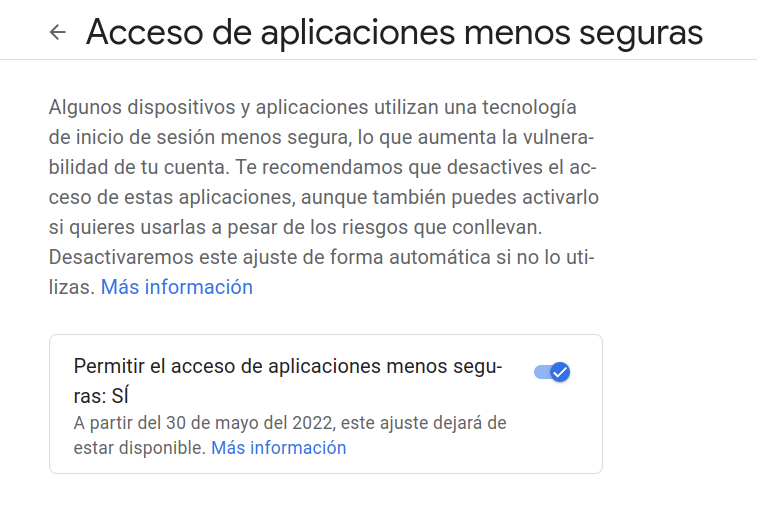
\includegraphics[scale=0.40]{imagenes/apps-access.png}
        \caption{Acceso de aplicaciones menos seguras}
        \label{fig:apps-access}
    \end{figure}

Como vemos, esta opción no parece muy recomendable ya que puede ser un punto vulnerable
en la seguridad de nuestra cuenta y de nuestra aplicación, por lo que finalmente se ha
decidido activar la autenticación en dos pasos y crear una contraseña de aplicación,
que estará en una variable de entorno junto al correo de la cuenta.

    \begin{figure}[H]
        \centering
        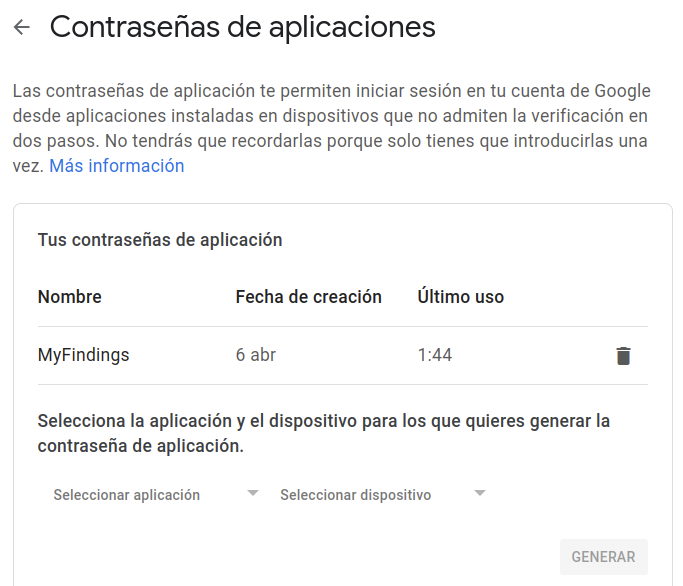
\includegraphics[scale=0.35]{imagenes/apps-pass.png}
        \caption{Contraseñas de aplicaciones}
        \label{fig:apps-pass}
    \end{figure}

\subsubsection{Permisos y roles de usuario}
Uno de los puntos más importantes de la aplicación es el manejo de permisos y roles de
usuario. Para el control de ello, Django viene integrado con un sistema de permisos,
que nos permite controlar qué usuarios pueden \textbf{ver}, \textbf{añadir}, \textbf{
modificar} o \textbf{eliminar}. Por ejemplo, para el manejo de los usuarios que pueden
realizar acciones sobre excavaciones tendríamos:

    \begin{itemize}
        \item \textbf{Ver}: controlar qué usuarios pueden ver excavaciones desde las
        vistas.
    % % DESCOMENTAR
    % \begin{minted}[mathescape, linenos,numbersep=5pt,bgcolor=lightgray,gobble=2,
    %        frame=lines,fontsize=\footnotesize,framesep=2mm]{python}
    % @login_required
    % @permission_required('myFindings.view_excavation', 
    %                                     raise_exception=True)
    % def list_allexcavations(request):
    %     # Get all excavations
    %     excavations = Excavation.objects.all()
    %     data = { 'excavations': excavations}
    
    %     return render(request, 'excavations_list.html', data)
    % \end{minted}

        \item \textbf{Añadir}: controlar qué usuarios pueden añadir excavaciones
        desde las vistas.
    % % DESCOMENTAR
    % \begin{minted}[mathescape, linenos,numbersep=5pt,bgcolor=lightgray,gobble=2,
    %        frame=lines,fontsize=\footnotesize,framesep=2mm]{python}
    % @login_required
    % @permission_required('myFindings.add_excavacion', 
    %                                     raise_exception=True)
    % def add_excavation(request):
    %     # Get the fields of excavation
    %     data = { 'form': ExcavationForm() }
    
    %     if request.method == 'POST':
    %         # Get the data entered by the user
    %         form = ExcavationForm(data=request.POST)
    %         if(form.is_valid()):    # Check if valid
    %             form.save()         # Save form
    
    %             # Redirect to the list of excavations
    %             return redirect(to='excavations')
    %         else:
    %             data['form'] = form
    
    %     return render(request, 'add_excavation.html', data)
    % \end{minted}

        \item \textbf{Modificar}: controlar qué usuarios pueden modificar excavaciones
        desde las vistas.
    % % DESCOMENTAR
    % \begin{minted}[mathescape, linenos,numbersep=5pt,bgcolor=lightgray,gobble=2,
    %        frame=lines,fontsize=\footnotesize,framesep=2mm]{python}
    % @login_required
    % @permission_required('myFindings.change_excavation', 
    %                                     raise_exception=True)
    % def modify_excavation(request, id):
    %     excavation = get_object_or_404(Excavation, id=id)
        
    %     # Guardar el formulario con los datos del cuadro
    %     data = { 'form': ExcavationForm(instance=excavation) }
    
    %     if request.method == 'POST':
    %         form = ExcavationForm(data=request.POST,
    %                                     instance=excavation)
    %         if form.is_valid():       # Si es válido
    %             form.save()           # Guardarlo
    
    %             return redirect(to="excavations")
    
    %         data["form"] = form
    
    %     return render(request, 'modify_excavation.html', data)
    % \end{minted}

        \item \textbf{Eliminar}: controlar qué usuarios pueden eliminar excavaciones
        desde las vistas.
    % % DESCOMENTAR
    % \begin{minted}[mathescape, linenos,numbersep=5pt,bgcolor=lightgray,gobble=2,
    %        frame=lines,fontsize=\footnotesize,framesep=2mm]{python}
    % @login_required
    % @permission_required('myFindings.delete_excavation',
    %                                     raise_exception=True)
    % def delete_excavation(request, id):
    %     # Get the excavation, if it doesn't exist, get an Http404
    %     excavation = get_object_or_404(Excavation, id=id)
    
    %     # Delete the excavation
    %     excavation.delete()    
    
    %     return redirect(to="excavations")
    % \end{minted}
    \end{itemize}

Como vemos, en todas las vistas se hace uso de \textbf{decoradores} \cite{decorators},
que nos permiten controlar el acceso a las vistas. En este caso, el decorador
\textbf{@login\_required} nos permite controlar que el usuario esté autenticado,
y el decorador \textbf{@permission\_required} nos permite controlar que el usuario
tenga el permiso correspondiente.\\

Esto hace mucho más segura la aplicación, ya que si un usuario no autenticado intenta
acceder a alguna url a la que no tiene permiso \textbf{escribiéndola directamente en
el navegador}, primero se comprobará que esté autenticado en el sistema, y en caso
contrario se le redirigirá a la página de login. Como vemos en la siguiente imagen,
el usuario ha intentado acceder a la página add\_excavation/ sin estar autenticado,
por lo que se le ha redirigido a la página de login para luego redirigirlo a la página
requerida (\textbf{?next=/add\_excavation/}).

    \begin{figure}[H]
        \centering
        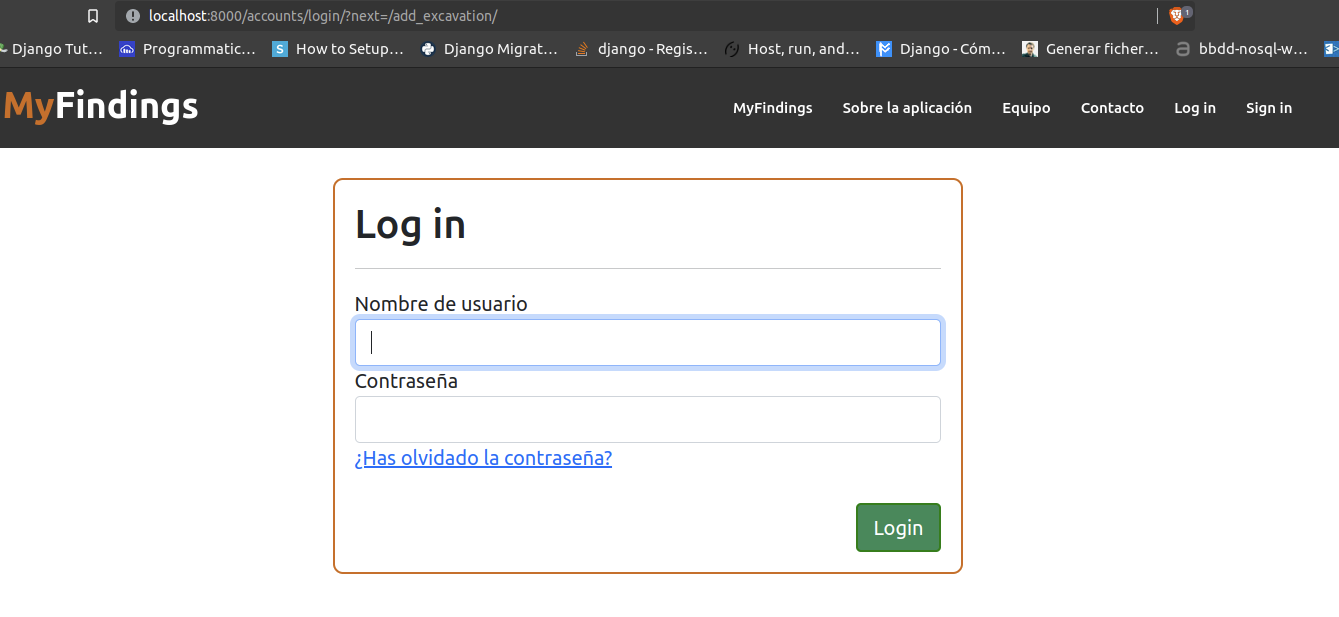
\includegraphics[scale=0.25]{imagenes/login-required.png}
        \caption{Login requerido}
        \label{fig:login-required}
    \end{figure}


Una vez autenticado, se pasará al segundo decorador, que comprobará que tenga el permiso
correspondiente y en caso contrario mostrará un mensaje de \textbf{403 Forbidden}

    \begin{figure}[H]
        \centering
        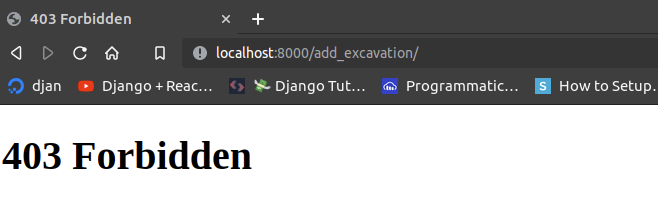
\includegraphics[scale=0.50]{imagenes/403-forbidden.png}
        \caption{Permiso denegado}
        \label{fig:403-forbidden}
    \end{figure}

Otro de los temas importantes de la aplicación son los roles de usuario, que serían los
siguientes:

    \begin{enumerate}
        \item \textbf{Administrador}: es el usuario que tiene todos los permisos del
        sistema, puede realizar cualquier acción dentro de él: eliminar modelos, eliminar
        usuarios, crear grupos, cambiar permisos a usuarios concretos, etc.
        \item \textbf{Staff}: es el usuario con permisos otorgados por el administrador
        del sistema. En nuestra aplicación corresponderá al arqueólogo con permisos
        privilegiados, que se encarga de aceptar o rechazar a los usuarios que se han
        enviado la petición de registro. Éstos deberán poder d \textbf{añadir y eliminar}
        usuarios de los grupos de permisos ya definidos, además de \textbf{tener acceso a
        todos los modelos} definidos en el sistema: excavaciones, inclusiones, materiales, etc.
        \item \textbf{Usuario registrado}: es el usuario común de la aplicación, que tendrá
        los permisos otorgados por el arqueólogo administrador (staff), bien por añadirlo
        a un \textbf{grupo de permisos} o por darle permisos específicos.
    \end{enumerate}
